% !TEX root = ./AM3C-Slides_annotations.1.tex
\documentclass["AM3C-Slides_annotations.tex"]{subfiles}

% \tikzset{external/force remake=true} % - remake all

\begin{document}

% \graphicspath{{\subfix{./.build/figures/AM3C-Slides_annotations.1}}}
% \tikzsetexternalprefix{./.build/figures/AM3C-Slides_annotations.1/graphics/}

\mymakesubfile{1}[AM 3C]
{Equações Diferenciais Ordinárias (EDO)} % Subfile Title
{Equações Diferenciais Ordinárias (EDO)} % Part Title

\begin{minipage}{60em}
  \begin{sectionBox}*1{All differential equation methods} % Sindex

    \begin{minipage}{40em}
      \subsection*{Ordinary first order equations}
      \begin{tcolorbox}
        \begin{align*}
          % \formulas-AM3C-EDO-linear-ordem-1
          y' + a(x)\,y &= b(x)
          & \text{EDO ord:1 (\ref{sec:edo ord:1 simple method})}
          ; \\
          % \formulas-AM3C-EDO-linear-ordem-1
          y' + a(x)\,y &= b(x)
          & \text{Method varying of arbitrary constants for edo ord:1 (\ref{sec:met solve diffeq ord:1 constvar})}
          ; \\
          % \formulas-AM3C-EDO-bernoulli
          y' + a(x)\,y &= b(x)\,y^k
          & \text{Bernoulli's equation (\ref{sec:bernoullis equation})}
          ; \\
          % \formulas-AM3C-EDO-Riccati
          y' + a(x)\,y &= b(x) + c(x)\,y^2
          & \text{Riccati's equation (\ref{sec:riccatis equation})}
        \end{align*}
      \end{tcolorbox}
    \end{minipage}
    
    \begin{minipage}{60em}
      \subsection*{General differential equations}
      \begin{tcolorbox}
        \begin{align*}
          P\,y &= 0
          ;&
          y &= \varphi(x)\,\prim_x{z}
          & \text{Order reduction of diffeq (\ref{sec:met order reduction})}
          % 
          % 
          % 
          ; \\
          P\,y &= 0
          &&& \text{Method of variation of arbitrary constants for n (\ref{sec:met arbconstvar ord:n})}
          % 
          % 
          % 
          ; \\
          P\,y &= e^{\alpha\,x}\,f(x)
          ; &
          y &= y_h + \bar{y}
          ; & \text{linear diffeq ord:n \(\mdif[n]{x} \to r^i\) (\ref{sec:linear diffeq ord:n constcoeff})}
          % 
          % 
          % 
          ; \\
          P\,y &= 0
          ; &
          y &= y_h
          ; & \text{linear diffeq ord:n \(\mdif[n]{x} \to r^i; f(x)=0\) (\ref{sec:linear diffeq constcoeff f=0})}
          % 
          % 
          % 
          ; \\
          P\,y &= e^{\alpha\,x}\,P_k(x)
          ; &
          \bar{y} &= x^p\,e^{\alpha\,x}\,Q_k(x)
          ; & \text{linear diffeq ord:n \(\mdif[n]{x} \to r^i; f=P_k(x)\) (\ref{sec:linear diffeq constcoef f=Pk})}
          % 
          % 
          % 
          ; \\
          P\,y &= e^{\alpha\,x}\,(a\,\cos(w\,x)+b\,\sin(w\,x))
          ; &
          \bar{y} &= x^p\,e^{\alpha\,x}\,(a_0\,\cos(w\,x)+b_0\,\sin(w\,x))
          ; & \text{linear diffeq ord:n \(\mdif[n]{x} \to r^i\) (\ref{sec:linear diffeq constcoef ord:n f=acos(wx)+bsin(wx)})}
          % 
          % 
          % 
          ;\\
          P\,y
          &= y\,\sum_{i=0}^{n}{a_i\,x^i\,\mdif[i]{x}}
          = f(x)
          = &
          = & y\,\sum_{i=0}^{n}{b_i\,\mdif[i]{t}}
          = f(e^t)
          ; x=e^t
          ; &
          \text{Eulers equation (\ref{sec:eulers equation})}
        \end{align*}
      \end{tcolorbox}
    \end{minipage}
    
    \begin{minipage}{60em}
      \subsection*{non-linear exact/non-exact equations}
      \begin{tcolorbox}
        \begin{align*}
          \begin{pmatrix}
            + u(x,y)\,\odif{x} 
            \\
            + v(x,y)\,\odif{y}
          \end{pmatrix}
          &= 0
          ; &
          \pdv{u}{y} &= \pdv{v}{x}
          ; &
          &&
          \text{exact (\ref{sec:nlinear exact diffeq})}
          % 
          % 
          % 
          ; \\
          \phi(x,y)
          \,\begin{pmatrix}
            + u(x,y)\,\odif{x} 
            \\
            + v(x,y)\,\odif{y}
          \end{pmatrix}
          &= 0
          ; &
          \pdv{(u\,\phi)}{y} &= \pdv{(v\,\phi)}{x}
          ; &
          &&
          \text{non-exact w integrating factor (\ref{sec:nlinear nexact diffeq integrating factor})}
          % 
          % 
          % 
          ; \\
          \begin{pmatrix}
            + u(x)\,\odif{x} 
            \\
            + v(y)\,\odif{y}
          \end{pmatrix}
          &= 0
          ; &
          \pdv{u}{y} &= \pdv{v}{x}
          ; & 
          \prim_x{u(x)} + \prim_y{v(y)} &= \text{const}
          ; & 
          \text{exact w sep variables (\ref{sec:nlinear exact diffeq separable variables})}
        \end{align*}
      \end{tcolorbox}
    \end{minipage}

    \begin{minipage}{40em}
      \subsection*{First order equations not solved by the derivative}
      \begin{tcolorbox}
        \begin{align*}
          y &= x\,\alpha(y') + \beta(y')
          ; &
          \alpha(y') &\neq y'
          ; &
          y'&=p
          ; & \text{Lagrange's equation (\ref{sec:lagranges equation})}
          % 
          % 
          % 
          ; \\
          y &= x\,y' + \beta(y')
          && &
          y'&=p
          ; & \text{Clairaut's equation (\ref{sec:clairauts equation})}
        \end{align*}
      \end{tcolorbox}
    \end{minipage}

    
    \begin{minipage}{30em}
    \subsection*{linear eqsystem of constcoeff} % Sindex
      \begin{tcolorbox}
        \begin{align*}
          \begin{Bmatrix}
            P_{x,0}\,x + P_{y,0}\,y &=& f_0(t)
            \\
            P_{x,1}\,x + P_{y,1}\,y &=& f_1(t)
            \\
            \dots
          \end{Bmatrix}
        \end{align*}
      \end{tcolorbox}
    \end{minipage}

  \end{sectionBox}\end{minipage}

\begin{sectionBox}1m{EDO de Primeira Ordem} % S1

  \begin{BM}
    F(x,y(x),y'(x)) = 0
  \end{BM} 
  \textit{F} é definida num conjunto aberto \(D\subset\mathbb{R}^3\).
  Dado um intervalo aberto \(I\subset\mathbb{R}\), Diz-se que uma função \(\phi:I\to\mathbb{R}\) diferenciavel em \textit{I} é uma solução da equação diferencial acima se:
  \begin{enumerate}
    \item \((x,\phi(x),\phi'(x))\in D, \quad \forall\,x\in I\)
    \item \(F(x,\phi(x),\phi'(x)) = 0, \quad \forall\,x\in I\)
  \end{enumerate}
  
  \paragraph*{Ordem de uma equação diferencial} é a ordem da derivada mais elevada referida na equação

  \begin{multicols}{2}
    \begin{exampleBox}1b{} % E1.1
      A equação
      \begin{BM}
        y' - \frac{y}{x} = x\,e^x
      \end{BM}
      é de primeira ordem e as funções
      \begin{BM}[align*]
        y(x) &= c\,x + x\,e^x & c\in\mathbb{R}
      \end{BM}
      são soluções em \(\myrange*{0,\infty}\) desta equação.
    \end{exampleBox}

    \begin{exampleBox}1b{} % E1.2
      A equação
      \begin{BM}
        y" + 4\,y = 0
      \end{BM}
      é de segunda ordem e as funções
      \begin{BM}[align*]
        y(x) &= c_1\,\cos{2\,x} 
        \\   &+ c_2\,\sin{2\,x},
        \\ & c_1,c_2\in\mathbb{R}
      \end{BM}

      São soluções em \(\mathbb{R}\) desta equação
    \end{exampleBox}
  \end{multicols}

  \subsection*{Forma normal}
  \begin{BM}
    y'(x) = f(x,y(x))
  \end{BM}
  Com \textit{f} definida no conjunto aberto \(A\subset\mathbb{R}^2\).
  As equações de primeira ordem na forma normal admitem uma interpretação geométricas relativamente simples e que \emph{permite ter uma ideia aproxiamada dos gráficos das soluções} destas esquações.
  
  \subsection*{Campo de direções da equação}
  Com uma equação diferencial de primeira ordem na forma normal definida no conjunto aberto \(A\subset\mathbb{R}^2\), se a cada ponto \((x,y)\) de \textit{A} se associar a direção das retas de declive igual a \(f(x,y)\), se obtem aquilo a que usualmente se chama de campo de direções da equação.

  \begin{exampleBox}1b{Campo de direções da equação} % E1.3
    \begin{BM}
      y'=-y
    \end{BM}
    \begin{center}
      % \tikzset{external/remake next=true}
      % \pgfplotsset{height=7cm, width= .6\textwidth}
      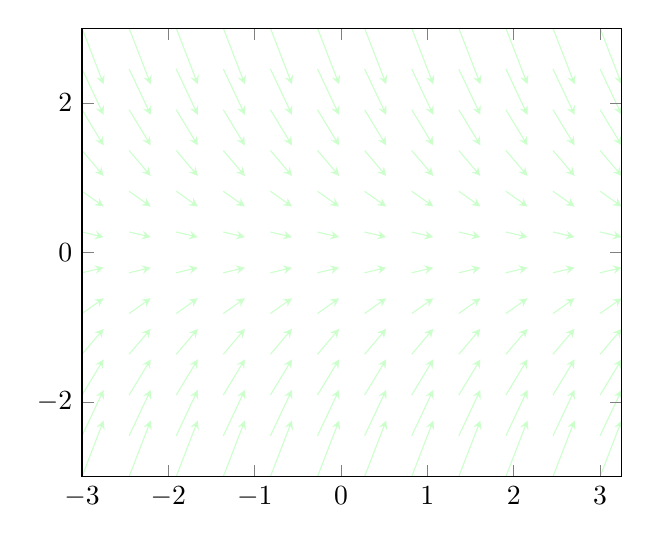
\begin{tikzpicture}
      \begin{axis}
        [
          % xmajorgrids = true,
          % legend pos={south east},
          xtick distance=1,
          domain=-3:3,
          y domain = -3:3,
          % ymin=-3.5,ymax=3.5,
          % xmin=-3.5,xmax=3.5,
          view={0}{90},
          % xlabel={},
          % ylabel={},
          % axis lines={center}, % left|right|center|box,
        ]

        % Plot from equation
        \addplot3[
          % opacity=1,
          opacity=0.2,
          \Graph{green},
          samples = 12,
          quiver = {
            u={1},
            v={-y},
            scale arrows=0.25,
          },
          -stealth,
        ]{0};
      \end{axis}
      \end{tikzpicture}
    \end{center}
    
  \end{exampleBox}
\end{sectionBox}

\begin{sectionBox}1m{Equação autonoma} % S2
  Uma EDO em que não aparece explicitamente a variável independente.
  Se for \textit{y} a função icógnita e \textit{x} a variável independente, uma equa;cão diferencial autónoma de primeira ordem é uma equação da forma \(F(y,y')=0\) ou na forma normal:
  \begin{BM}
    \odv{y}{x}=f(y)
  \end{BM}
  \paragraph*{Pontos de equilíbrio (críticos ou estacionários)} são os zeros da função 
  \begin{BM}
    f(c)=0 \implies y(x)=c \text{ é solução de } f(x)=\odv{y}{x}
  \end{BM}
  \(y(x)=c\) chama-se solução de equilíbrio (ou estacionária)


  \subsection*{Classificação dos pontos de equilíbrio (Eq autónomas)}
  Prestando atenção nos limites:
  \begin{BM}
    f(c)=0
  \end{BM}
  \begin{align*}
       x &\to +\infty          && \implies y(x) \to c \implies c \text{ é um ponto de eq estável}
    \\ x &\to -\infty          && \implies y(x) \to c \implies c \text{ é um ponto de eq instável}
    \\ x &\to -\infty \land x \to +\infty && \implies y(x) \to c \implies c \text{ é um ponto de eq semiestável}
  \end{align*}
\end{sectionBox}

\begin{exampleBox}1m{Pontos de equilíbrio} % E4
  Considere-se a equação autónoma
  \begin{BM}
    \odv{y}{x}=y(a-b\,y); a,b\in\mathbb{R}^+
  \end{BM}
  Pontos de equilíbrio:
  \begin{gather*}
    c=y:
    y(a-b\,y) = 0
    \begin{cases}
      y=0\\ y=\frac{a}{b}
    \end{cases}
    \\
    \therefore y(x)=0\lor y(x)=a/b
    \end{gather*}
  Podemos prever o comportamento da equalção pela seguinte tabela
  \begin{center}
    \vspace{1ex}
    \def\-{\cellC{Graph33}{-}}
    \def\+{\cellC{Graph32}{+}}
    \begin{tabular}{*{4}{C}}
      \toprule

      \multirow[c]{2}{*}{\(y\)} 
      & \multicolumn{3}{C}{sign}
      \\\cline{2-4}
      & y & a-b\,y & y(a-b\,y)

      \\\midrule

      y<0     & \- & \+ & \-
      \\ 0<y<a/b & \+ & \+ & \+
      \\ a/b<y   & \+ & \- & \-

      \\\bottomrule
    \end{tabular}
    \vspace{2ex}
  \end{center}
  Se desenharmos um grafico das soluções de equilíbrio
  \begin{center}
    % \tikzset{external/remake next=true}
    % \pgfplotsset{height=7cm, width= .6\textwidth}
    \begin{tikzpicture}
      \begin{axis}
        [
          % xmajorgrids = true,
          legend pos={south east},
          domain=-3:3,
          ymax=2,
          ymin=-1,
          xmax=3,
          xlabel={\(x/b\)},
          ylabel={\(y*b/a\)},
          axis lines={center}, % left|right|center|box,
          view={0}{90},
        ]
        % Legends
        % \addlegendimage{empty legend}
        % \addlegendentry[Graph]{\(
        %   {\color{Graph}x}
        %   {\color{GraphC}x^2}
        % \)}
        \addplot3[
            Graph!20!background,
            opacity=1,
            -stealth,
            samples=16,
            % domain=-2:2,
            quiver={
              u={1},
              v={y*(1-y)},
              scale arrows=0.150,
            },
          ](x,y,0);

        % Plot from equation
        \addplot[
            smooth,
            thick,
            Graph,
            samples = 2,
          ]{ 1 }
          node[above,pos=0.6,opacity=1]{\(y(x)=a/b\)};
        \addplot[
            smooth,
            thick,
            Graph,
            samples = 2,
          ]{ 0 }
          node[above,pos=0.6,opacity=1]{\(y(x)=0\)};

        \draw[-,ultra thick,Graph33] (0,-1) -- node[right]{-} (0,0);
        \draw[-,ultra thick,Graph32] (0, 0) -- node[right]{+} (0,1);
        \draw[-,ultra thick,Graph33] (0, 1) -- node[right]{-} (0,2);


        % y(a-by)
        % \frac{y}{b/a}(a-b\,y*a/b)
        % \frac{y}{b}(1-y)

        % English
        % 19:00 % marcação
        % 808 204 020 % geral


      \end{axis}
    \end{tikzpicture}
  \end{center}
  Podemos ver que as tres regiões divididas pelos dois pontos de equilíbrio tem um comportamento: \(R_1\) Decrescente, \(R_2\) Crescente e \(R_3\) Decrescente\\
  Seja \(y(x)=0\) a solução que verifica a condição inicial \(y(0)=y_0\):
  \begin{align*}
    y_0 &< 0
    && \begin{cases}
      x \to -\infty &\implies y(x) \to 0
      \\ x \to +\infty &\implies y(x) \to -\infty
    \end{cases}
    \\
    0 < y_0 &< a/b
    && \begin{cases}
      x \to -\infty &\implies y(x) \to 0
      \\ x \to +\infty &\implies y(x) \to a/b
      % y(x) \to_{+} 0 \impliedby x \to -\infty
      % \\ y(x) \to_{-} a/b \impliedby x \to +\infty
    \end{cases}
    \\
    a/b < y_0 &
    && \begin{cases}
      x \to -\infty &\implies y(x) \to +\infty
      \\ x \to +\infty &\implies y(x) \to a/b
      % y(x) \to_{+} a/b \impliedby x \to +\infty
    \end{cases}
  \end{align*}
  Podemos dizer que \(y(x)=0\) é um ponto de equilíbrio instável e que \(y(x)=a/b\) é um ponto de equilíbrio estável
\end{exampleBox}
\begin{exampleBox}1m{Equilíbrio semiestável} % E6
  A equação autónoma
  \begin{BM}
    \odv{y}{x} = (y-1)^2
  \end{BM}
  tem \(y=1\) como único ponto de equilíbrio. Observando a reta fase, verifica-se que qualquer solução \(y(x)\) em qualquer um dos intervalos \(\myrange*{-\infty,1}\text{ e }\myrange*{1,+\infty}\) é crescente
  \begin{center}
    % \tikzset{external/remake next=true}
    % \pgfplotsset{height=7cm, width= .6\textwidth}
    \begin{tikzpicture}
      \begin{axis}
        [
          % xmajorgrids = true,
          % legend pos={south east},
          domain=-3:3,
          ymax=2,
          ymin=-1,
          % xmax=3,
          % xlabel={\(x/b\)},
          % ylabel={\(y*b/a\)},
          axis lines={center}, % left|right|center|box,
          view={0}{90},
        ]
        % Legends
        % \addlegendimage{empty legend}
        % \addlegendentry[Graph]{\(
        %   {\color{Graph}x}
        %   {\color{GraphC}x^2}
        % \)}
        \addplot3[
            Graph!20!background,
            opacity=1,
            -stealth,
            samples=24,
            % y domain=-0.5:2,
            quiver={
              u={1},
              v={(y-1)^2},
              scale arrows=0.150,
            },
          ](x,y,0);

        % Plot from equation
        \addplot[
            smooth,
            thick,
            Graph,
            % domain=-2:2,
            samples=2,
          ] {1}
          node[above,pos=0.6,opacity=1]{\(y(x)=1\)};

      \end{axis}
    \end{tikzpicture}
  \end{center}
  Podemos caracterizar esse ponto como \emph{ponto de equilíbrio semiestável}
\end{exampleBox}

\begin{sectionBox}*2m{Soluções implicitas e explicitas} % S
  \begin{multicols}{2}
    \begin{sectionBox}*2{Soluções explicitas}
      \begin{BM}
        y = f(x)
      \end{BM}
      \textit{y} isolado
    \end{sectionBox}

    \begin{sectionBox}*2{Soluções implicitas}
      \begin{BM}
        G(x,y)=0
      \end{BM}
      Define implicitamente uma função \(y(x)\) solução da equação.
    \end{sectionBox}
  \end{multicols}

  \begin{exampleBox}1b{} % E
    Da equação
    \begin{BM}
      y^2\,y'=x^2
    \end{BM}
    Podemos tirar a solução de duas formas
    \begin{multicols}{2}
      \begin{minipage}{0.4\textwidth}
        Da forma implicita
        \begin{BM}
          y^3 -x^3 -8 = 0
        \end{BM}
      \end{minipage}

      \begin{minipage}{0.4\textwidth}
        Da forma explicita
        \begin{BM}
          y = \varphi(x) = \sqrt[3]{8+x^3}
        \end{BM}
      \end{minipage}
    \end{multicols}
  \end{exampleBox}
\end{sectionBox}

\begin{sectionBox}*2m{Famílias de Soluções} % S
  \begin{BM}
    G(x,y,z) = 0
  \end{BM}
  Tal como sucede no cálculo da primitiva de uma função, em que aparece uma constante \textit{c} de integração, \emph{quando se resolve uma EDO de primeira ordem, geralmente obtém-se com solução uma expressão contendo uma constante (ou parâmetro) \textit{c}, e que representa um conjunto de soluções} a que se chamará família de soluções a um parâmetro.

  \paragraph*{Soluções particulares} são obtidas quando atribuimos valores ao parametro da familia de soluções

  \paragraph*{Solucções singulares} nem sempre existem mas existem, não podem ser obtidas atribuindo um valor a constante \textit{c}

  \paragraph*{Integral Geral} Uma família de soluções que define todas as soluções de uma EDO para um intervalo \textit{I}
\end{sectionBox}

\begin{sectionBox}1m{Equação Linear de Primeira Ordem} % S2
  \label{sec:edo ord:1 simple method}
  \begin{BM}
    y' = f(x,y)
    \iff y' + p(x)y = q(x)
  \end{BM}
  Com \(p(x)\) e \(q(x)\) funções contínuas num intervalo aberto \(I \subseteq \mathbb{R}\)

  \begin{exampleBox}*1b{Exemplo} % E
    \begin{flalign*}
      y' + 2\,x\,y = x^3
      \begin{cases}
        p(x) = 2\,x
        \\ q(x) = x^3
      \end{cases}
    \end{flalign*}
  \end{exampleBox}

  \subsection*{Equação linear homgénea}
  Equação linear em que \(q(x) = 0\), quando em uma equação linear completa (\(q(x) \neq 0 \land p(x) \neq 0\)) substituirmos \(q(x)\) por 0, obtemos a equação linear homogénea associada.
\end{sectionBox}

\begin{sectionBox}*2m{Solução geral de equações lineáres de primeira ordem} % S
  \begin{BM}
    y' + a(x)\,y = b(x)
  \end{BM}

  % tag  = 3.w
  % a(x) = a(x)
  % b(x) = b(x)
  % y    = y
  % x    = x

  General solution
  \begin{tcolorbox}
    \begin{gather*}
      y
      = \frac{c_0}{\varphi(x)}
      + \frac{1  }{\varphi(x)}
      \,\int{b(x)\,\varphi(x)\,\odif{x}}
      %
      %
      %
      = \mathText{using 
        \eqref{eq:3.w phi_x}
        \eqref{eq:3.w prim}
      }
      = \dots
      %
      \yesnumber\label{eq:3.w answer}
    \end{gather*}
  \end{tcolorbox}

  Finding \(\varphi(x)\)
  \begin{tcolorbox}
    \begin{gather*}
      \varphi(x) 
      = \exp{\left(
          \int{a(x)\,\odif{x}}
      \right)}
      = \dots
      %
      \yesnumber\label{eq:3.w phi_x}
    \end{gather*}
  \end{tcolorbox}

  Integrating
  \begin{tcolorbox}
    \begin{gather*}
      \prim_x{\left(
          b(x)\,\varphi(x)
      \right)}
      = \mathText{using \eqref{eq:3.w phi_x}}
      = \dots
      %
      \yesnumber\label{eq:3.w prim}
    \end{gather*}
  \end{tcolorbox}

  \begin{sectionBox}*3b{Demonstração} % Sindex
    \begin{gather*}
      y' + p(x)\,y = q(x)
      \implies
      \left(
        y' + p(x)\,y 
      \right)\,\varphi(x)
      = \\
      = y'\,\exp{\left(\int{p(x)\,\odif{x}}\right)}
      + p(x)\,y\,\exp{\left( \int{p(x)\,\odif{x}} \right)}
      = \left(
        y\,\exp{\int{p(x)\,\odif{x}}}
      \right)'
      = \\
      = q(x)\,\varphi(x)
      = q(x)\,\exp{\int{p(x)\,\odif{x}}}
      \implies \\
      \implies y\,\exp{\int{p(x)\,\odif{x}}}
      = c+\int{
        q(x)\,\exp{\left(\int{p(x)\,\odif{x}}\right)}
        \,\odif{x}
      }
      \implies \\
      \implies y
      = \frac{c}{\exp{\int{p(x)\,\odif{x}}}}
      + \frac{1}{\exp{\int{p(x)\,\odif{x}}}}
      \,\int{
        q(x)\,\exp{\left(\int{p(x)\,\odif{x}}\right)}
        \,\odif{x}
      }
      = \\
      = \frac{c}{\varphi(x)}
      + \frac{1}{\varphi(x)}
      \,\int{q(x)\,\varphi(x)\,\odif{x}}
    \end{gather*}
  \end{sectionBox}

\end{sectionBox}

\begin{exampleBox}1m{} % E
  Considere a equação
  \begin{BM}
    y' + (1-1/x)\,y = 2\,x 
    ,\quad x < 0
  \end{BM}
  Encontre a solução para a equação acima e a equação homgénea associada

  \answer{}

  % tag  = 7
  % a(x) = (1-1/x)
  % b(x) = 2\,x
  % y    = y
  % x    = x
  \begin{gather*}
    y
    = \frac{c_0}{\varphi(x)}
    + \frac{1  }{\varphi(x)}
    \,\int{2\,x\,\varphi(x)\,\odif{x}}
    %
    %
    %
    = \mathText{using \eqref{eq:7-phi_x}}
    = \frac{c_0}{(e^{x}\,c_2/x)}
    + \frac{1  }{(e^{x}\,c_2/x)}
    \,\int{2\,x\,(e^{x}\,c_2/x)\,\odif{x}}
    %
    %
    %
    = \mathText{using \eqref{eq:7-prim}}
    = c_3\,x\,e^{-x}
    + \frac{x  }{e^{x}\,c_2}
    \,2\,c_2\,e^{x}
    = c_3\,x\,e^{-x}
    + 2\,x
  \end{gather*}

  % φ(x)
  \begin{gather*}
    \varphi(x) 
    = \exp{\left(
      \int{(1-1/x)\,\odif{x}}
    \right)}
    = \exp{
      x
      - \ln{x}
      + c_1
    }
    = e^{x}\,c_2/x
    %
    \yesnumber\label{eq:7-phi_x}
  \end{gather*}

  % prim
  \begin{gather*}
    P\left(
      2\,x\,\varphi(x)
    \right)
    = \mathText{using \eqref{eq:7-phi_x}}
    = P\left(
      2\,x\,e^{x}\,c_2/x
    \right)
    = 2\,c_2\,e^{x}
    %
    \yesnumber\label{eq:7-prim}
  \end{gather*}

\end{exampleBox}

\begin{exampleBox}1m{} % E8
  Na investigação de um homicídio, é, muitas vezes importante estimar o instante em que a morte ocorreu. A partir de observações experimentais, a lei de arrefecimento de Newton estabelece, com uma exatidão satisfatória, que a taxa de variação da temperatura \(T(t)\) de um corpo em arrefecimento é proporcional à diferença entre a temperatura desse corpo e a temperatura constante \(T_a\) do meio ambiente, isto é:
  \begin{BM}
    \odv{T}{t} = -k\,(T-T_a)
    %
    \yesnumber\label{eq:8-dTdt}
  \end{BM}
  Suponhamos que duas horas depois a temperatura é novamente medida e o valor encontrado é \(T_1 = \qty*{23}{\celsius}\). O crime parece ter ocorrido durante a madrugada e corpo foi encontrado pela manhã bem cedo, pelas 6 horas e 17 minutos. A perícia então faz a suposição adicional de que a temperatura do meio ambiente entre a hora da morte e a hora em que o cadáver foi encontrado se manteve mais ou menos constante nos 20°C. A perícia sabe também que a temperatura normal de um ser humano vivo é de 37°C. Vejamos como, com os dados considerados, a perícia pode determinar a hora em que ocorreu o crime.

  \answer{}

  Encontrando tempo de morte
  \begin{tcolorbox}
    \begin{gather*}
      t:T(t) = 37
      %
      \yesnumber\label{eq:8-T=37}
      \cong \mathText{using \eqref{eq:8 t(t)}}
      \cong 10\,e^{-t\,\num{0.601986402162968}}
      + 20
      \implies
      t 
      \cong -\ln(1.7)/\num{0.601986402162968}
      \cong \qty{-0.881462187776328}{\hour}
      \cong \qty{-52.887731266579699}{\minute}
    \end{gather*}
  \end{tcolorbox}

  Desenvolvendo \eqref{eq:8-dTdt}
  \begin{tcolorbox}
    \begin{gather*}
      \odv{T}{t} 
      = -k\,(T-T_a)
      = -k\,T+k\,T_a
      = -k\,T+k\,20
      \implies
      \odv{T}{t}
      + k\,T
      = k\,20
      %
      \yesnumber\label{eq:8-dTdt 2}
    \end{gather*}
  \end{tcolorbox}

  % tag  = 8
  % a(x) = k
  % b(x) = k\,20
  % y    = T
  % x    = t

  Solução geral \(T(t)\) a partir de \eqref{eq:8-dTdt 2}
  \begin{tcolorbox}
    \begin{gather*}
      T
      = \frac{c_0}{\varphi(t)}
      + \frac{1  }{\varphi(t)}
      \,\int{k\,20\,\varphi(t)\,\odif{t}}
      %
      %
      %
      = \mathText{using 
        \eqref{eq:8 phi_x}
        \eqref{eq:8-prim}
      }
      = \frac{c_0}{c_1\,e^{k\,t}}
      + \frac{1  }{c_1\,e^{k\,t}}
      k\,20\,c_1\,\left(
        c_2+e^{k\,t}/k
      \right)
      = (c_0/c_1)\,e^{-k\,t}
      + c_2\,k\,20\,e^{-k\,t}
      + 20
      = \\
      = c_3\,e^{-k\,t}
      + 20
      %
      \yesnumber\label{eq:8 T(t c_3 k)}
      \cong \mathText{using \eqref{eq:8 c_3}\eqref{eq:8 k}}
      \cong 10\,e^{-t\,\num{0.601986402162968}}
      + 20
      %
      \yesnumber\label{eq:8 t(t)}
    \end{gather*}
  \end{tcolorbox}

  Encontrando constantes \(k,c_3\)
  \begin{tcolorbox}
    % k
    \begin{gather*}
      T(2) = 23
      = \mathText{using \eqref{eq:8 T(t c_3 k)}\eqref{eq:8 c_3}}
      = 10\,e^{-k\,2}
      + 20
      \implies
      k 
      = -\ln(0.3)/2
      \cong \num{0.601986402162968}
      %
      \yesnumber\label{eq:8 k}
      % 
      % 
      % 
      ;\\
      T(0) = 30
      = \mathText{using \eqref{eq:8 T(t c_3 k)}}
      = c_3\,e^{-k*0}
      + 20
      = c_3
      + 20
      \implies
      c_3 = 10
      % 
      \yesnumber\label{eq:8 c_3}
    \end{gather*}
  \end{tcolorbox}

  Resolvendo \(\varphi(x)\)
  \begin{tcolorbox}
    % φ(x)
    \begin{gather*}
      \varphi(t) 
      = \exp{\left(
          \int{k\,\odif{t}}
      \right)}
      = c_1\,e^{ k\,t }
      %
      \yesnumber\label{eq:8 phi_x}
    \end{gather*}
  \end{tcolorbox}

  Integrando
  \begin{tcolorbox}
    \begin{gather*}
      P\left(
        k\,20\,\varphi(t)
      \right)
      = \mathText{using \eqref{eq:8 phi_x}}
      = P\left(
        k\,20\,c_1\,e^{k\,t}
      \right)
      = k\,20\,c_1\,\left(
        c_2+e^{k\,t}/k
      \right)
      %
      \yesnumber\label{eq:8-prim}
    \end{gather*}
  \end{tcolorbox}

\end{exampleBox}

\begin{sectionBox}1m{Método de Variação das constantes Eq Diff de ordem 1} % S
  \label{sec:met solve diffeq ord:1 constvar}
  Um metodo alternativo para resolver a mesma equação diferencial linear de primeira ordem
  \begin{BM}
    y' + a(x)\,y = b(x)
  \end{BM}

  Solução geral
  \begin{gather*}
    y 
    = \frac{C(x)}{\varphi(x)}
    %
    \yesnumber\label{eq:4 y(C(x))}
    = \mathText{using
      \eqref{eq:4 C(x)}
      \eqref{eq:4 phi_x}
    }
    = \dots
  \end{gather*}

  Finding \(C(x)\)
  \begin{gather*}
    y' + a(x)\,y 
    = \mathText{using \eqref{eq:4 y(C(x))}}
    = \mdif{x}{\left(
        \frac{C(x)}{\varphi(x)}
    \right)}
    + a(x)
    \,\frac{C(x)}{\varphi(x)}
    = b(x)
    \implies C'(x) = \dots
    \implies
    C(x) = \dots
    %
    \yesnumber\label{eq:4 C(x)}
  \end{gather*}

  Finding \(\varphi(x)\)
  \begin{gather*}
    \varphi(x)
    = \exp{\left(
        \prim_x{\left(
            a(x)
        \right)}
    \right)}
    = \dots
    %
    \yesnumber\label{eq:4 phi_x}
  \end{gather*}

  Podemos resolver a equação homogênea associada \(y_h\) substituir \(c_0 \to c_0(x)\) e aplicar \(y=c_0(x)/\varphi(x)\) na equação linear original, dessa forma podemos obter \(c_0(x)\) e por sequencia \(y=c_0(x)/\varphi{x}\)

  \section*{Método usando solução particular}
  \begin{BM}
    y 
    = \frac{c_0}{\varphi(x)}
    + \frac{1  }{\varphi(x)}
    \,\int{q(x)\,\varphi(x)\,\odif{x}}
    = y_h + y_i
  \end{BM}
  \begin{itemize}
    \item \(y_h\) é a solução da equação homogênea associada
    \item \(y_i\) é uma solução particular
  \end{itemize}
  Mesmo \(y_i\) aparecer como uma solução particular em que \(c_0=1\), por estarmos trabalhando com uma solução arbitrária, isso não impede de ser qualquer solução particular, da no mesmo ao final das contas
\end{sectionBox}

\begin{exampleBox}1m{} % E

  \begin{BM}
    y' - \frac{2x}{x^2+1}\,y = 1
  \end{BM}
  Encontre a solução geral usando o método de variação das constantes
  
  \answer{}

  Solução geral
  \begin{tcolorbox}
    \begin{gather*}
      y
      = \frac{C(x)}{\varphi(x)}
      %
      \yesnumber\label{eq:e.9 y(C(x))}
      = \mathText{using
        \eqref{eq:e.9 C(x)}
        \eqref{eq:e.9 phi_x}
      }
      = \frac{
        c_1\,(
          \arctan{x}+c_2
        )    
      }{
        \frac{c_1}{x^2+1}
      }
      = \left(x^2+1\right)
      \,\left(
        \arctan{x}
        + c_2
      \right)
    \end{gather*}
  \end{tcolorbox}

  Finding \(C(x)\)
  \begin{tcolorbox}
    \begin{gather*}
      y'-\frac{2\,x}{x^2+1}
      = \mathText{using 
        \eqref{eq:e.9 y(C(x))}
        \eqref{eq:e.9 phi_x}
      }
      = \mdif{x}{\left(
          \frac{C(x)}{\frac{c_1}{x^2+1}}
      \right)}
      - \frac{2\,x}{x^2+1}
      \,\frac{C(x)}{\frac{c_1}{x^2+1}}
      % = \\
      = \frac{1}{c_1}\left(
        C'(x)
        (x^2+1)
        + C(x)\,2\,x
      \right)
      - \frac{C(x)\,2\,x}{c_1}
      = \\
      = C'(x)\,\frac{x^2+1}{c_1}
      = 1
      % \implies \\
      \implies
      C'(x) 
      = \frac{c_1}{x^2+1}
      \implies \\
      \implies
      C(x)
      = \prim_x{\left(
          \frac{c_1}{x^2+1}
      \right)}
      = c_1\,(
        \arctan{x}+c_2
      )    
      %
      \yesnumber\label{eq:e.9 C(x)}
    \end{gather*}
  \end{tcolorbox}
  
  Finding \(\varphi(x)\)
  \begin{tcolorbox}
    \begin{gather*}
      \varphi(x)
      = \exp{\left(
          \prim_x{\left(
              -\frac{2\,x}{x^2+1}
          \right)}
      \right)}
      = \exp{\left(
          -\int{\left(
              \frac{\odif{x^2+1}}{x^2+1}
          \right)}
      \right)}
      = \\
      = \exp{\left(
          -(
            \ln(x^2+1)+c_0
          )
      \right)}
      = 
      \frac{c_1}{x^2+1}
      %
      \yesnumber\label{eq:e.9 phi_x}
    \end{gather*}
  \end{tcolorbox}

\end{exampleBox}

\begin{sectionBox}1m{Equação de Bernoulli e a equação de Riccati} % S5
  São equações não lineares que, após mudanças de variáveis apropriadas, se transformam em equações lineares:

  \subsection{Eq de Bernoulli}
  \label{sec:bernoullis equation}
  \begin{BM}
    \shortintertext{A atribuição}
    y = z^{1/(1-k)}
    \shortintertext{Transforma a eq diferencial}
    y' + a(x)\,y = b(x)\,y^k
    \implies
    z' + (1-k)\,a(x)\,z = (1-k)\,b(x)
    \shortintertext{onde \(z\) pode ser encontrado por}
    z 
    = \frac{c_0}{\varphi(x)}
    + \frac{1  }{\varphi(x)}
    \,\int{(1-k)\,b(x)\,\varphi(x)\,\odif{x}}
    ; \\
    \varphi(x)
    = \exp{\left(
        \int{(1-k)\,a(x)\,\odif{x}}
    \right)}
  \end{BM}
  Quando encontramos uma EDO que possa ser escrita na forma acima, podemos realizar a substituiçãp de \(z=y^{1-k}\) transformando a EDO em uma equação linear, assim podemos encontrar a solução geral para \textit{z} que pode ser substituida para encontrar a solução de \textit{y} que é a equação original.

  \begin{sectionBox}*3b{workflow} % S
    \begin{BM}
      y' + a(x)\,y = b(x)\,y^k
    \end{BM}

    Solução geral
    \begin{tcolorbox}
      \begin{gather*}
        y = z^{1/(1-k)}
        = \left(
          \frac{c_0}{\varphi(x)}
          + \frac{1}{\varphi(x)}
          \,\int{(1-k)\,b(x)\,\varphi(x)\,\odif{x}}
        \right)^{1/(1-k)}
        = \mathText{using 
          \eqref{eq:w 5.1 phi_x}
          \eqref{eq:w 5.1 prim}
        }
        = \dots
      \end{gather*}
    \end{tcolorbox}
    
    Encontrando \(\varphi(x)\)
    \begin{tcolorbox}
      \begin{gather*}
        \varphi(x)
        = \exp{\left(
            \int{(1-k)\,a(x)\,\odif{x}}
        \right)}
        = \dots
        %
        \yesnumber\label{eq:w 5.1 phi_x}
      \end{gather*}
    \end{tcolorbox}

    Resolvendo integral
    \begin{tcolorbox}
      \begin{gather*}
        \int{(1-k)\,b(x)\,\varphi(x)\,\odif{x}}
        = \mathText{using \eqref{eq:w 5.1 phi_x}}
        = \dots
        %
        \yesnumber\label{eq:w 5.1 prim}
      \end{gather*}
    \end{tcolorbox}
    
  \end{sectionBox}

  \subsection{Eq de Riccati}
  \label{sec:riccatis equation}
  \begin{BM}
    \shortintertext{A substituição}
    y = y_1 + 1/z
    \shortintertext{Transforma a eq diferencial}
    y' + a(x)\,y = b(x) + c(x)\,y^2
    \implies \\
    \implies z' + (2\,c(x)\,y_1-a(x))z = -c(x)
    \shortintertext{onde \(z\) pode ser encontrado por}
    z
    = \frac{c_0}{\varphi(x)}
    + \frac{  1}{\varphi(x)}
    \,\int{
      -c(x)\,\varphi(x)\,\odif{x}
    }
    ; \\
    \varphi(x)
    = \exp{\left(
        \int{
          \left(
            2\,c(x)\,y_1
            -a(x)
          \right)
          \,\varphi(x)
          \,\odif{x}
        }
    \right)}
  \end{BM}
\end{sectionBox}

\begin{exampleBox}1m{Eq de Bernoulli} % E
  
  Considere o problma de valores iniciais (PVI)
  \begin{BM}[align*]
    y' - x\,y = x\,y^3 
    ,\quad 
    y(0) = 1
  \end{BM}

  \answer{\eqref{eq:e.10 answer}}

  % tag= e.10
  % a(x) = (-x)
  % b(x) = x
  % k    = 3

  Substituição de Bernoulli
  \begin{tcolorbox}
    \begin{gather*}
      y = z^{1/(1-3)}
      \implies
      y' - x\,y = x\,y^3 
      % \implies \\
      \implies
      z' + (1-k)\,(-x)\,z = (1-k)\,3
    \end{gather*}
  \end{tcolorbox}
  
  Solução geral
  \begin{tcolorbox}
    \begin{gather*}
      y 
      = z^{1/(1-3)}
      = \left(
        \frac{c_0}{\varphi(x)}
        +\frac{1 }{\varphi(x)}
        \,\int{
          (1-3)\,x
          \,\varphi(x)
          \,\odif{x}
        }
      \right)^{-1/2}
      = \mathText{using
        \eqref{eq:e.10 phi_x}
        \eqref{eq:e.10 prim}
      }
      = \left(
        \frac{c_0}{c_2\,e^{x^2}}
        +\frac{1 }{c_2\,e^{x^2}}
        (-c_2)
        \,\left(
          e^{x^2}+c_3
        \right)
      \right)^{-1/2}
      = \left(
        c_5\,e^{-x^2}
        -1
      \right)^{-1/2}
      %
      \yesnumber\label{eq:e.10 y(x c_5)}
      = \mathText{using \eqref{eq:e.10 c_5}}
      = \left(
        2\,e^{-x^2}
        -1
      \right)^{-1/2}
      %
      \yesnumber\label{eq:e.10 answer}
    \end{gather*}
  \end{tcolorbox}

  Encontrando \(c_5\)
  \begin{tcolorbox}
    \begin{gather*}
      y(0)=1
      = \mathText{using \eqref{eq:e.10 y(x c_5)}}
      = \left(
        c_5\,e^{-0^2}
        -1
      \right)^{-1/2}
      \implies \\
      \implies
      c_5 = 1+1^2 = 2
      %
      \yesnumber\label{eq:e.10 c_5}
    \end{gather*}
  \end{tcolorbox}
  
  Encontrando \(\varphi(x)\)
  \begin{tcolorbox}
    \begin{gather*}
      \varphi(x)
      = \exp{\left(
          \prim_x\left(
            (1-3)\,(-x)
          \right)
      \right)}
      = \exp{\left(
          2(c_1+x^2/2)
      \right)}
      = c_2\,e^{x^2}
      % 
      \yesnumber\label{eq:e.10 phi_x}
    \end{gather*}
  \end{tcolorbox}
  
  Integrando
  \begin{tcolorbox}
    \begin{gather*}
      \int{
        (1-3)\,x
        \,\varphi(x)
        \,\odif{x}
      }
      = \mathText{using \eqref{eq:e.10 phi_x}}
      = -\int{
        2\,x
        \,c_2\,e^{x^2}
        \,\odif{x}
      }
      = -c_2
      \,\int{
        e^{x^2}
        \,\odif{\left( x^2 \right)}
      }
      = -c_2
      \,\left(
        e^{x^2}+c_3
      \right)
      % 
      \yesnumber\label{eq:e.10 prim}
    \end{gather*}
  \end{tcolorbox}
  
\end{exampleBox}

\begin{exampleBox}1m{Eq Bernoulli} % E
  Suponhamos que numa comunidade constituida por \textit{N} individuos
  \begin{itemize}
    \item \(y(t)\) representa o número de intectados pelo vírus da gripe A
    \item \(x(t)=N-y(t)\) representa a população não infectada.
  \end{itemize}
  Considere-se que o vírus se propaga pelo contacto entre infectados e não infectados e que a propagação é proporcional ao número de contactos entre estes dois grupos. Suponhamos também que os elementos dos dois grupos se relacionam livremente entre si de modo que o número de contactos entre infectados e não infectados é proporcional ao produto de \(x(t)\) por \(y(t)\) isto é
  \begin{BM}
    k\,x(t) = k\,(N-y(t))\,y(t)
  \end{BM}
  em que \textit{k} é a constante de proporcionalidade.
  se \(y_0\) é o numero inicial de infectados, o número de infectados \(y(t)\) no instante \(t\) é a solução PVI
  \begin{BM}[align*]
    y' &= k\,(N-y)\,y 
    ;& k &> 0
    ;& y(0) = y_0
  \end{BM}

  \answer{}

  Incompleta:
  \begin{gather*}
      y: 
      y' = k\,(N-y)\,y 
      \implies
      y' - N\,k\,y = -k\,y^2 
      % 
      % 
      % 
      ; \\[1ex]
      y 
      = z^{-1}
      = \left(
        c\,e^{-N\,k\,t}
        + \frac{1}{N\,t}
      \right)^{-1}
      = \dots
      = \frac{N\,y_0}
      { (N-y_0)\,e^{-N\,k\,t} + y_0 }
      % 
      % 
      % 
      ; \\[1ex]
      c: 
      y(0)^{-1}
      = (z(0))
      = c\,e^{-N\,k *0}
      + \frac{1}{N *0}
      = y_0^{-1}
      % 
      % 
      % 
      ; \\[1ex]
      % a(t) = (-N\,k)
      % b(t) = (-k)
      % k    = 2
      z=y^{1-2}  = 1/y
      \implies \\
      \implies
      z' + N\,k\,z = k
      % a(t) = N\,k
      % b(t) = k
      % y    = z
      % x    = t
      z
      = \frac{c_0}{\varphi(t)}
      + \frac{1  }{\varphi(t)}
      \,\int{k\,\varphi(t)\,\odif{t}}
      %
      %
      %
      = \\[1ex]
      = \frac{c_0}{c_2\,e^{N\,k\,t}}
      + \frac{1  }{c_2\,e^{N\,k\,t}}
      \,\int{k\,c_2\,e^{N\,k\,t}\,\odif{t}}
      % 
      = e^{-N\,k\,t}
      \,\frac{c_0}{c_2}
      + e^{-N\,k\,t}
      \,\frac{k\,c_2}{c_2}
      \,\frac{e^{N\,k\,t}}{N\,k\,t}
      = c\,e^{-N\,k\,t}
      + \frac{1}{N\,t}
      ;\\
      c = c_0/c_2
      %
      %
      %
      ; \\[1ex]
      \varphi(t) 
      = \exp{\left(
        \int{N\,k\,\odif{t}}
      \right)}
      = \exp{\left(
        N\,k\,t+c_1
      \right)}
      = c_2\,e^{N\,k\,t}
      ; \\ c_2 = e^{c_1}
    \end{gather*}
\end{exampleBox}

\begin{exampleBox}1m{Eq Riccati} % E12

  Determine a solução do PVI
  \begin{BM}
    y' - y = -2\,x + \frac{1}{2\,x^2}\,y^2
    ,\quad y(1) = -2
    ,\quad x > 0
  \end{BM}
  Sabendo que a equação admite a solução \(y=2\,x\)

  % tag  = e.12
  % a(x) = (-1)
  % b(x) = (-2\,x)
  % c(x) = \frac{1}{2\,x^2}
  % y_1(x) = 2\,x

  \answer{\eqref{eq:e.12 answer}}

  Riccati substitution
  \begin{tcolorbox}
    \begin{gather*}
      y = 2\,x + z^{-1}
      \implies
      y' + (-1)\,y = (-2\,x) + \frac{1}{2\,x^2}\,y^2
      \implies \\
      \implies
      z' + \left(2\,\frac{1}{2\,x^2}\,2\,x - (-1)\right)\,z 
      = z' + (1+2/x)\,z 
      = -\frac{1}{2\,x^2}
    \end{gather*}
  \end{tcolorbox}
  
  General solution
  \begin{tcolorbox}
    \begin{gather*}
      y
      = 2\,x + z^{-1}
      = 2\,x + \left(
        \frac{c_0}{\varphi(x)}
        + \frac{1}{\varphi(x)}
        \,\prim_x{\left(
            -\frac{1}{2\,x^2}
            \,\varphi(x)
        \right)}
      \right)^{-1}
      = \mathText{using
        \eqref{eq:e.12 phi_x}
        \eqref{eq:e.12 prim}
      }
      = 2\,x + \left(
        \frac{c_0}{e^x\,x^2\,c_3}
        + \frac{1}{e^x\,x^2\,c_3}
        \frac{-c_3}{2}\,\left( e^x+c_4 \right)
      \right)^{-1}
      = 2\,x + \left(
        \frac{c_6}{e^{x}\,x^{2}}
        - \frac{1}{2\,x^2}
      \right)^{-1}
      %
      \yesnumber\label{eq:e.12 y(x c_6)}
      = \mathText{using \eqref{eq:e.12 c_6}}
      = 2\,x + \left(
        \frac{e/4}{e^{x}\,x^{2}}
        - \frac{1}{2\,x^2}
      \right)^{-1}
      %
      \yesnumber\label{eq:e.12 answer}
    \end{gather*}
  \end{tcolorbox}

  Finding \(c_6\)
  \begin{tcolorbox}
    \begin{gather*}
      y(1)=-2
      = \mathText{using \eqref{eq:e.12 y(x c_6)}}
      = 2*1 + \left(
        \frac{c_6}{e^{1}\,1^{2}}
        - \frac{1}{2*1^2}
      \right)^{-1}
      = 2 + \left(
        \frac{c_6}{e}
        - \frac{1}{2}
      \right)^{-1}
      \implies \\
      \implies
      c_6
      = e\left(
        (-2-2)^{-1}
        + \frac{1}{2}
      \right)
      = \frac{e}{4}
      % 
      \yesnumber\label{eq:e.12 c_6}
    \end{gather*}
  \end{tcolorbox}

  Finding \(\varphi(x)\)
  \begin{tcolorbox}
    \begin{gather*}
      \varphi(x)
      = \exp{\left(
          \prim_x{(
              1+2/x
          )}
      \right)}
      = \exp{\left(
          x
          +c_1
          +2\,(
            c_2 + \ln{x}
          )
      \right)}
      = 
      e^x\,x^2\,c_3
      %
      \yesnumber\label{eq:e.12 phi_x}
    \end{gather*}
  \end{tcolorbox}

  Integrating
  \begin{tcolorbox}
    \begin{gather*}
      \prim_x{\left(
          -\frac{1}{2\,x^2}
          \,\varphi(x)
      \right)}
      = \mathText{using \eqref{eq:e.12 phi_x}}
      = \prim_x{\left(
          -\frac{1}{2\,x^2}
          \,e^x\,x^2\,c_3
      \right)}
      = -\frac{c_3}{2}
      \,\prim_x{\left(
          e^x
      \right)}
      = 
      -\frac{c_3}{2}\,\left( e^x+c_4 \right)
      %
      \yesnumber\label{eq:e.12 prim}
    \end{gather*}
  \end{tcolorbox}
  
\end{exampleBox}

\begin{sectionBox}1m{Operador de Derivação \(\mdif{}\)} % S
  \begin{BM}
    \mdif[n]{x} = \odv[n]{}{x}
    \\
    \mdif[k]{x} :C^n(I) \to C^{n-k}(I)
    \\ \mdif[k]{x} : y \to y^{(k)}=\odv[k]{y}{x}
  \end{BM}
\end{sectionBox}

\begin{sectionBox}1m{Equação Diferencial Linear de ordem \textit{n}} % S
  \begin{BM}[align*]
    \sum_{i=0}^n{
      a_i\,\mdif[i]{x}(y)
    } 
    = \left(\sum_{i=0}^n{
        a_i\,\mdif[i]{x}
    }\right)\,y
    = P\,y
    = f(x)
  \end{BM}

  \begin{itemize}
    \item \(a_n\) é o Coeficiente lider
    \item Forma normal é quando esta escrita de forma que \(a_n=1\)
  \end{itemize}

  \begin{exampleBox}*1b[-4ex]{Example} % Eindex
    \begin{BM}
      \mdif[3]{x}(y) + x^2\,\mdif[2]{x}(y) - 5\,x\,\mdif[1]{x}(y) + y = x\,\cos(x)
    \end{BM}
    está escrita na forma normal
  \end{exampleBox}
\end{sectionBox}

\begin{sectionBox}*2m{Operador P} % Sindex

  \begin{BM}
    P = \mdif[n]{x} + \sum_{i=0}^{n-1}{
      a_{i}\,\mdif[i]{x}
    }
  \end{BM}

  \subsection*{Linearidade}
  Dadas duas funções \(y_1,y_2 \in C^n(I)\) e \(\alpha,\beta\) numeros reais
  \begin{BM}
    P(\alpha\,y_1 + \beta\,y_2) = \alpha\,P\,y_1 + \beta\,P\,y_2
  \end{BM}

  \subsection*{Espaço Solução da equação}
  \begin{BM}
    \nuc(P) : A = \{  y \in C^n(I) : P\,y = 0 \}
  \end{BM}
  O conjunto á é nucleo do operador P, sendo portanto um subespaço de \(C^n(I)\). Este subespaço é designado por espaço solução da equação

  \subsection*{Teorema: Solução que satisfaz \(P\,y=0\)}
  \begin{BM}
    y=\varphi(x) : \mdif[i]{x}\varphi(x_0) = \alpha_i
    \\ x_0 \in I
    \land \alpha_i \in \mathbb{R}\quad \forall\,i
  \end{BM}
  Dado um \(x_0\) no intervalo aberto \textit{I} e constantes reais arbitrarias \(\alpha\), existe uma e só uma função que satisfaz \(P\,y=0\)

  \subsection*{Finidade da dimensão de \(\nuc(P)\)}
  \begin{BM}
    \dim(\nuc(P)) = n \impliedby P = \mdif[n]{x} + \sum_{i=0}^{n-1}{a_i\,\mdif[i]{x}}
  \end{BM}m
  Sendo o espaço solução da equação \(P\,y = 0\) (\(\nuc(P)\)) um subespaço do espaço liear \(C^n(I)\), Não limitado a ter dimenção infinita, a dimensão do nucleo de \textit{P} deve ser \textit{n} (limitado).

  \subsection*{Solução trivial}
  \begin{BM}
    \alpha_i=0\quad\forall\,i 
    \impliedby \\
    \impliedby
    \sum_{i=0}^{n}{\alpha_i\,y_i(x)} = 0 
    : \{y\}\text{ é linearmente idependente}
  \end{BM}

  \section*{Sistema fundamental de soluções de \(P\,y = 0\)}
  \begin{BM}
    y = \sum_{i=1}^{n}{c_i\,y_i}
  \end{BM}
  \begin{itemize}
    \item \(\{y_i\,\forall\,i\}\) é um sistema fundamental de soluções de \(P\,y = 0\)
    \item \(c_i\,\forall\,i\) são constantes arbitrárias que consituem a sua solução (ou integral) geral
  \end{itemize}
  Quaisquer \textit{n} soluções linearmente idependentes de \(P\,y=0\) que constituem uma base de \(\nuc(P)\)

\end{sectionBox}

\begin{sectionBox}1m{Abaixando a ordem de uma EDO} % Sindex
  \label{sec:met order reduction}
  \begin{BM}
    z(x) : y = \varphi(x)\,\int{(z)\,\odif{x}}
    ;\\ P\,y=0
  \end{BM}
  \begin{itemize}
    \item \(\varphi(x)\) é uma solução particular da equação linear homogenea de ordem \textit{n} (\(P\,y = 0\))
  \end{itemize}
\end{sectionBox}

\begin{exampleBox}1m{Baixamento de grau de uma Eq lin homogenea} % E13
  Determine a solução geral da equação
  \begin{BM}
    y'' + y'/x-y/x^2 = 0
    ,\quad x>0
  \end{BM}
  Sabendo que \(\varphi(x) = x\) é uma solução.
  
  \answer{}

  Solução geral
  \begin{tcolorbox}
    \begin{gather*}
      y
      = \varphi(x)\,\prim_x{(z)}
      = x\,\prim_x{(z)}
      % 
      \yesnumber\label{eq:e.13 y->z}
      = \mathText{using \eqref{eq:e.13 z(x)}}
      = x\,\prim_x{\left(
          \frac{c_3}{x^3} 
      \right)}
      = x\,c_3\,\left(\frac{1}{2\,x^2}+c_4\right)
      = \frac{c_5}{x}+x\,c_6
    \end{gather*}
  \end{tcolorbox}
  
  Substitution \(y \to z\)
  \begin{tcolorbox}
    \begin{gather*}
      y'' + y'/x-y/x^2 = 0
      \implies \mathText{using
        \eqref{eq:e.13 y->z}
        \eqref{eq:e.13 Dx(y)}
        \eqref{eq:e.13 D2x(y)}
      }
      \implies
      (
        2\,z + x\,z'
      )
      + \frac{1}{x}(
        \prim_x{(z)} + x\,z
      )
      - \frac{1}{x^2}(
        x\,\prim_x{(z)} 
      )
      = \\
      = 2\,z 
      + x\,z'
      + \prim_x{(z)}/x
      + z
      - \prim_x{(z)}/x
      % = \\
      = x\,z' + 3\,z 
      = 0
      \implies
      z' + \frac{3}{x}\,z = 0
      % 
      \yesnumber\label{eq:e.13 eq z}
    \end{gather*}
  \end{tcolorbox}
  
  Finding \(\mdif[1]{x}{y},\mdif[2]{x}{y}\)
  \begin{tcolorbox}
    \begin{gather*}
      \mdif{x}{y}
      = \mathText{using \eqref{eq:e.13 y->z}}
      = \mdif{x}{\varphi(x)}
      \,\prim_x{(z)}
      + \varphi(x)\,z
      = \mdif{x}{\varphi(x)}
      \,\prim_x{(z)}
      + \varphi(x)\,z
      = 
      \prim_x{(z)} + x\,z
      % 
      \yesnumber\label{eq:e.13 Dx(y)}
      ;\\
      \mdif[2]{x}{y}
      = \mathText{using \eqref{eq:e.13 Dx(y)}}
      = \mdif{x}{(\prim_x{(z)} + x\,z)}
      = 
      2\,z + x\,z'
      % 
      \yesnumber\label{eq:e.13 D2x(y)}
    \end{gather*}
  \end{tcolorbox}

  Solving \eqref{eq:e.13 eq z}
  \begin{tcolorbox}
    \begin{gather*}
      z
      = c_0\,(\varphi_z(x))^{-1}
      = c_0\,\left(
        \exp{\left(
            \int{(3/x)\,\odif{x}}
        \right)}
      \right)^{-1}
      = c_0\,\left(
        e^{3\,(\ln{(x)}+c_1)}
      \right)^{-1}
      = c_0\,(
        c_2\,x^3
      )^{-1}
      = \\
      = 
      \frac{c_3}{x^3} 
      %
      \yesnumber\label{eq:e.13 z(x)}
    \end{gather*}
  \end{tcolorbox}
  
\end{exampleBox}

\begin{sectionBox}1m{Wronskiano: check dependencia linear} % Sindex
  \begin{BM}[align*]
    W(f_1,f_2,\dots,f_n)(x)
    &= \det(w)
    ;&
    w \in \mathcal{M}_{n,m}
    : w_{i,j} &= \mdif[j]{x}\,f_i
  \end{BM}
  \vspace{-3ex}
  \begin{BM}
    W(f_1,f_2,\dots,f_n)(x)
    \begin{cases}
         = 0 &\text{ Linear depedent}
      \\ \neq 0 &\text{ Linear independent}
    \end{cases}
  \end{BM}

\end{sectionBox}

\begin{sectionBox}1m{Método de variação das constantes abitrárias para equação linear de ordem \textit{n}} % Sindex
  \label{sec:met arbconstvar ord:n}
  \begin{BM}[gather*]
      % a_0(x) = a_1(x)
      % a_1(x) = a_1(x)
      % a_2(x) = a_2(x)
      % a_3(x) = a_3(x)
      % f(x)   = f(x)
      % y_1(x) = y_1(x)
      % y_2(x) = y_1(x)
      % y_3(x) = y_1(x)
      y:
      \begin{pmatrix}
          a_1(x)
        \\ + a_1(x)\,\mdif[1]{x}
        \\ + a_2(x)\,\mdif[2]{x}
        \\ + a_3(x)\,\mdif[3]{x}
      \end{pmatrix}
      \,y
      = f(x)
      %
      %
      %
      \\[1ex]
      y
      = c_1(x)\,y_1(x)
      + c_2(x)\,y_2(x)
      + c_3(x)\,y_3(x)
      %
      %
      %
      \\[1ex]
      \begin{Bmatrix}
        {
            c_1'(x)\,\mdif[0]{x}y_1(x) 
          + c_2'(x)\,\mdif[0]{x}y_2(x)
          + c_3'(x)\,\mdif[0]{x}y_3(x)
        } = 0
        \\ {
            c_1'(x)\,\mdif[1]{x}\,y_1(x) 
          + c_2'(x)\,\mdif[1]{x}\,y_2(x)
          + c_3'(x)\,\mdif[1]{x}\,y_3(x)
        } = 0
        \\ {
            c_1'(x)\,\mdif[2]{x}\,y_1(x) 
          + c_2'(x)\,\mdif[2]{x}\,y_2(x)
          + c_3'(x)\,\mdif[2]{x}\,y_3(x)
        } = \frac{f(x)}{a_3(x)}
      \end{Bmatrix}
  \end{BM}
\end{sectionBox}

\begin{exampleBox}1m{Metodo das var const arb} % E14

  Considere a equação
  \begin{BM}
    y" + 9\,y = 1/\cos(3\,x)
    ;\quad x\in\myrange*{-\pi/6,\pi/6}
  \end{BM}
  As funções \(\cos{(3\,x)}\text{ e }\sin{(3\,x)}\) são duas soluções linearmente idependentes da equação homogénea
  \begin{BM}
    y'' + 9\,y = 0
  \end{BM}
  Pelo que seu integral geral será dado por
  \begin{BM}
    y = c_1\,\cos{(3\,x)} + c_2\,\sin{(3\,x)}
    ;\quad c_1,c_2\in\mathbb{R}
    \yesnumber\label{eq:e.14 y_h}
  \end{BM}
  Utilizemos o método da variação das constantes arbitrárias para determinar o integral geral da equação completa

  % tag    = 14
  % a_0(x) = 9
  % a_1(x) = 0
  % a_2(x) = 1
  % f(x)   = \frac{1}{\cos{(3\,x)}}

  \answer{\eqref{eq:e.14 answer}}

  General solution
  \begin{tcolorbox}
    \begin{gather*}
      y
      = \mathText{using \eqref{eq:e.14 y_h}}
      = C_1(x)\,y_1(x)
      + C_2(x)\,y_2(x)
      = \mathText{using
        \eqref{eq:e.14 C_1}
        \eqref{eq:e.14 C_2}
      }
      = \left(
        - \ln{(\cos(3\,x))} - c_3
      \right)
      \cos(3\,x)
      + \left(
        x/3 + c_4
      \right)
      \sin(3\,x)
      %
      \yesnumber\label{eq:e.14 answer}
    \end{gather*}
  \end{tcolorbox}

  Finding \(C_1(x),C_2(x)\)
  \begin{tcolorbox}
    \begin{gather*}
      C_1(x) 
      = \prim_x{(C_1'(x))}
      = \mathText{using \eqref{eq:e.14 C_1'}}
      = \prim_x{\left(
          3\,\frac
          {\sin{(3\,x)}}
          {\cos{(3\,x)}}
      \right)}
      = \mathText{using \(
          \odif{(\cos(3\,x))}
          = -\sin(3\,x)\,3\,\odif{x}
      \)}
      = -\int{\left(
          \frac
          {\odif{(\cos{(3\,x)})}}
          {\cos{(3\,x)}}
      \right)}
      = 
      - \ln{(\cos(3\,x))} - c_3
      % 
      \yesnumber\label{eq:e.14 C_1}
      % 
      % 
      % 
      ;\\
      C_2(x) 
      = \prim_x{(C_2'(x))}
      = \mathText{using \eqref{eq:e.14 C_2'}}
      = \prim_x{\left(
          1/3
      \right)}
      = x/3 + c_4
      % 
      \yesnumber\label{eq:e.14 C_2}
    \end{gather*}
  \end{tcolorbox}

  Finding \(C_1'(x),C_2'(x)\)
  \begin{tcolorbox}
    \begin{gather*}
      C_1'(x)
      = \mathText{using \eqref{eq:e.14 eq system}}
      = \left(
        W_{y_1,y_2}
      \right)^{-1}
      \,\begin{vmatrix}
        0 
        &  \mdif[0]{x}y_2
        \\ \frac{1}{\cos{(3\,x)}}
        &  \mdif[1]{x}y_2
      \end{vmatrix}
      = \mathText{using
        \eqref{eq:e.14 w}
        \eqref{eq:e.14 D1x(y_2)}
      }
      = \frac{1}{3}
      \,\begin{vmatrix}
        0 
        &  \sin{(3\,x)}
        \\ \frac{1}{\cos{(3\,x)}}
        &  3\,\cos{(3\,x)}
      \end{vmatrix}
      = 3\,\frac{\sin{(3\,x)}}{\cos{(3\,x)}}
      % 
      \yesnumber\label{eq:e.14 C_1'}
      % 
      % 
      % 
      ; \\
      C_2'(x)
      = \mathText{using \eqref{eq:e.14 eq system}}
      = \left(
        W_{y_1,y_2}
      \right)^{-1}
      \,\begin{vmatrix}
        \mdif[0]{x}y_1
        &  0 
        \\ \mdif[1]{x}y_1
        &  \frac{1}{\cos{(3\,x)}}
      \end{vmatrix}
      = \mathText{using
        \eqref{eq:e.14 w}
        \eqref{eq:e.14 D1x(y_1)}
      }
      = \frac{1}{3}
      \,\begin{vmatrix}
        \cos{(3\,x)}
        &  0 
        \\ -3\,\sin{(3\,x)}
        &  \frac{1}{\cos{(3\,x)}}
      \end{vmatrix}
      = 1/3
      % 
      \yesnumber\label{eq:e.14 C_2'}
    \end{gather*}
  \end{tcolorbox}

  Wronskiano
  \begin{tcolorbox}
    \begin{gather*}
      W(y_1,y_2)
      = \det\begin{bmatrix}
        \mdif[0]{x}\,y_1
        &  \mdif[0]{x}\,y_2
        \\ \mdif[1]{x}\,y_1
        &  \mdif[1]{x}\,y_2
      \end{bmatrix}
      =
      \mathText{using 
        \eqref{eq:e.14 D1x(y_1)}
        \eqref{eq:e.14 D1x(y_2)}
      }
      = \det\begin{bmatrix}
        \cos{(3\,x)}
        &  \sin{(3\,x)}
        \\ -3\,\sin{(3\,x)}
        &  +3\,\cos{(3\,x)}
      \end{bmatrix}
      = 3\,\cos^2{(3\,x)}
      +3\,\sin^2{(3\,x)}
      = 3
      % 
      \yesnumber\label{eq:e.14 w}
    \end{gather*}
  \end{tcolorbox}
  
  Equation system from Crammer's rule
  \begin{tcolorbox}
    \begin{gather*}
      \begin{Bmatrix}
        {
          c_1'(x)\,\mdif[0]{x}\,y_1(x) 
          + c_2'(x)\,\mdif[0]{x}\,y_2(x)
        } &=& 0
        \\ {
          c_1'(x)\,\mdif[1]{x}\,y_1(x) 
          + c_2'(x)\,\mdif[1]{x}\,y_2(x)
        } &=& \frac{1}{\cos{(3\,x)}}
      \end{Bmatrix}
      \yesnumber\label{eq:e.14 eq system}
    \end{gather*}
  \end{tcolorbox}

  Solving \(\mdif{x}{(y_1,y_2)}\)
  \begin{tcolorbox}
    \begin{gather*}
      \mdif[1]{x}{y_1}
      = \mdif[1]{x}\,\cos{(3\,x)}
      = -3\,\sin{(3\,x)}
      \yesnumber\label{eq:e.14 D1x(y_1)}
      %
      %
      ; \\
      \mdif[1]{x}{y_2}
      = \mdif[1]{x}\,\sin{(3\,x)}
      = +3\,\cos{(3\,x)}
      \yesnumber\label{eq:e.14 D1x(y_2)}
    \end{gather*}
  \end{tcolorbox}

\end{exampleBox}

\begin{sectionBox}1m{A equação linear de ordem \textit{n} de coeficientes consntantes} % S
  \label{sec:linear diffeq ord:n constcoeff}
  To find the solution for a diferential equation this method searches for the solutions for an associated polynom \(P(x) \to r\)

  \begin{BM}
    P(x)\,y = f(x)\,e^{\alpha\,x}
  \end{BM}

  General solution
  \begin{tcolorbox}
    \begin{gather*}
      y = y_h + \bar{y}
      = \mathText{using
        \eqref{eq:s.11 map polynom -> solution y}
        \land
        (
          \eqref{eq:s.11.1 bar y}
          \lor
          \eqref{eq:s.11.2 bar y}
        )
      }
      = \dots
    \end{gather*}
  \end{tcolorbox}

  Case 1: \(f(x) = P_k(x)\) polynom of order \(k\)
  \begin{tcolorbox}
    Solving for \(\bar{y}\)
    \begin{tcolorbox}
      \begin{gather*}
        \bar{y}
        = x^p\,e^{\alpha\,x}
        \,Q_k(x)
        = x^p\,e^{\alpha\,x}
        \,\sum_{i=0}^{k}{
          x^i\,\rho_i
        }
        = x^p\,e^{\alpha\,x}
        \,\left(
          x^0\,\rho_0
          x^1\,\rho_1
          x^2\,\rho_2
          x^3\,\rho_3
        \right)
        %
        \yesnumber\label{eq:s.11 bar y (x rho)}
        %
        = \mathText{using \eqref{eq:s.11 rho of bar y}}
        = \dots
        % 
        \yesnumber\label{eq:s.11.1 bar y}
      \end{gather*}
    \end{tcolorbox}

    Finding constants of \eqref{eq:s.11 bar y (x rho)}
    \begin{tcolorbox}
      \begin{gather*}
        \bar{y}\,P(x)
        = x^p\,e^{\alpha\,x}\,Q_k(x)
        \,P(x)
        = f(x)\,e^{\alpha\,x}
        \implies
        \begin{cases}
          \rho_0 = \dots
          \\ \rho_1 = \dots
          \\ \dots
        \end{cases}
        %
        \yesnumber\label{eq:s.11 rho of bar y}
      \end{gather*}
    \end{tcolorbox}
  \end{tcolorbox}

  Case 2: \(f(x) = (a\,\cos(w\,x)+b\,\cos(w\,x))\,e^{\alpha\,x}\)
  \begin{tcolorbox}
    Finding \(\bar{y}\)
    \begin{tcolorbox}
      \begin{gather*}
        \bar{y}
        = x^p\,(
          a_0\,\cos(w\,x)
          + b_0\,\sin(w\,x)
        )
        % 
        \yesnumber\label{eq:s.11 bar y of x a0 b0}
        = \mathText{using \eqref{eq:s.11 a0 b0 of bar y}}
        = \dots
        %
        \yesnumber\label{eq:s.11.2 bar y}
      \end{gather*}
    \end{tcolorbox}

    Finding constants of \eqref{eq:s.11 bar y of x a0 b0}
    \begin{tcolorbox}
      \begin{gather*}
        \bar{y}\,P(x)
        = x^p\,e^{\alpha\,x}\,(
          a_0\,\cos(w\,x)
          + b_0\,\sin(w\,x)
        )\,P(x)
        = \\
        = e^{\alpha\,x}\,\left(
          a\,\cos(w\,x)
          +b\,\cos(w\,x)
        \right)
        \implies \\
        \begin{cases}
          x^p\,a_0 = a 
          &\implies a_0 = \dots
          \\
          x^p\,b_0 = b
          & \implies
          b_0 = \dots
        \end{cases}
        % 
        \yesnumber\label{eq:s.11 a0 b0 of bar y}
      \end{gather*}
    \end{tcolorbox}
  \end{tcolorbox}

  Mapping \eqref{eq:s.11 roots} roots to solution of \(y_h\)
  \begin{tcolorbox}
    \label{sec:11 mapping roots to solution of y_h}
    \begin{gather*}
      \left\{
      \begin{align*}
        r_i &= \alpha_i
        & \to && 
        (\mdif[i]{x}-\alpha_i)^{q_i}
        && \to &&
        e^{r_i\,x}
        &
        \,\sum_{j=0}^{i-1}{
          a_{i,j}\,x^j
        }
        \\
        r_i &= \alpha_i \pm i\,\beta_i
        & \to &&
        ((\mdif[i]{x}-\alpha_i)^2-\beta_i^2)^{q_i}
        && \to &&
        e^{r_i\,x}
        &
        \,\begin{pmatrix}
          \cos(\beta_i\,x)
          \,\sum_{j=0}^{i-1}{
            a_{i,j,0}\,x^j
          }
          \\
          \sin(\beta_i\,x)
          \,\sum_{j=0}^{i-1}{
            a_{i,j,1}\,x^j
          }
        \end{pmatrix}
      \end{align*}
      \right.
      \vspace{10ex}
    \end{gather*}
    Examples
    \begin{gather*}
      \left\{
      \begin{align*}
        r_0 &= 2
        & \to && 
        (\mdif[i]{x}-2)^{1}
        && \to &&
        e^{2\,x}
        &
        \,a_{0,0}
        \\
        r_1 &= 3
        & \to && 
        (\mdif[i]{x}-3)^{4}
        && \to &&
        e^{3\,x}
        &
        \,\left(
          a_{1,0}\,x^0
          + a_{1,1}\,x^1
          + a_{1,2}\,x^2
          + a_{1,3}\,x^3
        \right)
        \\
        r_2 &= 4 \pm i\,1
        & \to &&
        ((\mdif[i]{x}-4)^2-1^2)^{1}
        && \to &&
        e^{4\,x}
        &
        \,\begin{pmatrix}
          \cos(1\,x) a_{2,0,0}
          \\
          \sin(1\,x) a_{2,0,1}
        \end{pmatrix}
        \\
        r_3 &= 2 \pm i\,2
        & \to &&
        ((\mdif[i]{x}-2)^2-2^2)^{2}
        && \to &&
        e^{2\,x}
        &
        \,\begin{pmatrix}
          \cos(2\,x)
          (
            a_{3,0,0}\,x^0
            + a_{3,1,0}\,x^1
          )
          \\
          \sin(2\,x)
          (
            a_{3,0,1}\,x^0
            + a_{3,1,1}\,x^1
          )
        \end{pmatrix}
      \end{align*}
      \right.
      % 
      \yesnumber\label{eq:s.11 map polynom -> solution y}
    \end{gather*}
  \end{tcolorbox}

  Associated polynom roots
  \begin{tcolorbox}
    \begin{gather*}
      P(x)
      = \mdif[n]{x}
      + \sum_{i=0}^{n-1}{\left(
          a_i\,\mdif[i]{x}
      \right)}
      \implies \\
      \implies
      r^n
      + \sum_{i=0}^{n-1}{\left(
          a_i\,r^i
      \right)}
      \implies \shortintertext{Finding solutions for \(r\)}
      \implies
      r = \begin{cases}
        \alpha_1 \pm i\,\beta_1,
        \\ \alpha_2 \pm i\,\beta_2,
        \\ \dots,
        \\ \alpha_n \pm i\,\beta_n,
      \end{cases}
      %
      \yesnumber\label{eq:s.11 roots}
      \implies \shortintertext{The solutions for \(r\) allows to rewrite the differential equation like so}
      \implies
      P(x)\,y
      = y
      \,\prod_{i=0}^n{
        (\mdif{i}-\alpha_i)
      }
      = f(x)\,e^{\alpha\,x}
    \end{gather*}
  \end{tcolorbox}
  In this format looking at \(\alpha\) and \(f(x)\) whe can find the general solution for \(y\) for specific cases, which include
  \begin{itemize}
    \item Homogeneous equation \(P(x)\,y=0\) \ref{sec:linear diffeq constcoeff f=0}
  \end{itemize}
\end{sectionBox}

\begin{sectionBox}2m{Quando \(f(x)=0\)} % Sindex
  \label{sec:linear diffeq constcoeff f=0}

  \begin{BM}
    P(x)\,y = 0
  \end{BM}

  General solution for \(y\)
  \begin{tcolorbox}
    \begin{gather*}
      P(x)\,y
      = \mathText{using 
        \eqref{eq:s.11 map polynom -> solution y}
        \eqref{eq:s.11.2 r_i}
      }
      = y
      \,\prod_i{\left(
          \mdif[i]{x}-\alpha_i
      \right)^{q_{r_i}}}
      \,\prod_i{\left(
          \left(\mdif[i]{x}-\alpha_i\right)^2
          -\beta_i^2
      \right)^{q_{r_i}}}
      \implies \mathText{using \eqref{eq:s.11 map polynom -> solution y}}
      \implies
      \dots
    \end{gather*}
  \end{tcolorbox}

  Map for polynom root \(\to\) solution for \(y\)
  

  Finding solutions for \eqref{eq:s.11.2 r polynom}
  \begin{tcolorbox}
    \begin{gather*}
      r = \{
        \alpha_1 \pm \beta_1,
        \alpha_2 \pm \beta_2,
        \dots,
        \alpha_n \pm \beta_n,
      \}
      % 
      \yesnumber\label{eq:s.11.2 r_i}
    \end{gather*}
    
  \end{tcolorbox}

  Associated polynom
  \begin{tcolorbox}
    \begin{gather*}
      P(x)
      = \mdif[n]{x}
      + \sum_{i=0}^{n-1}{
        a_i\,\mdif[i]{x}
      }
      \implies
      r^n
      + \sum_{i=0}^{n-1}{
        a_i\,r^i
      }
      %
      \yesnumber\label{eq:s.11.2 r polynom}
    \end{gather*}
  \end{tcolorbox}

\end{sectionBox}

\begin{exampleBox}1m{} % Eindex
  A equação diferencial linear de coeficientes constantes
  \begin{BM}
    (\mdif[2]{x}-2)
    (
      (\mdif{x}-2)^2
      + 9
    )^2
    \,y
    = 0
  \end{BM}
  Encontre a solução geral

  \answer{\eqref{eq:e.15 answer}}

  General solution
  \begin{tcolorbox}
    \begin{gather*}
      y
      = \mathText{using \eqref{eq:e.15 mapped roots}}
      = 
        e^{+\sqrt{2}\,x}\,c_1
      + e^{-\sqrt{2}\,x}\,c_2
      + e^{2\,x}
      \,\begin{pmatrix}
        + \cos(3\,x)
        (c_{3,0,0}+c_{3,1,0}\,x)
        \\
        + \sin(3\,x)
        (c_{3,0,1}+c_{3,1,1}\,x)
      \end{pmatrix}
      % 
      \yesnumber\label{eq:e.15 answer}
    \end{gather*}
  \end{tcolorbox}

  Mapping roots \eqref{eq:e.15 roots} to solution
  \begin{tcolorbox}
    \begin{gather*}
      \yesnumber\label{eq:e.15 mapped roots}
      r_1 = +\sqrt{2}
      \implies
      e^{+\sqrt{2}\,x}
      \,c_1
      ; \\
      r_2 = -\sqrt{2}
      \implies
      e^{-\sqrt{2}\,x}
      \,c_2
      ; \\
      r_3 = r_4 
      = 2\pm i\,3
      \implies
      e^{2\,x}
      \,\begin{pmatrix}
        + \cos(3\,x)
        (c_{3,0,0}+c_{3,1,0}\,x)
        \\
        + \sin(3\,x)
        (c_{3,0,1}+c_{3,1,1}\,x)
      \end{pmatrix}
    \end{gather*}
  \end{tcolorbox}

  Associated polynom
  \begin{tcolorbox}
    \begin{gather*}
      P(x)
      = (\mdif[2]{x}-2)
      (
        (\mdif{x}-2)^2
        + 9
      )^2
      \implies \\
      \implies
      (r^2-2)
      (
        (r-2)^2
        + 9
      )^2
      = (r-\sqrt{2})
      (r+\sqrt{2})
      (
        (r-2)^2
        + 3^2
      )^2
      \implies \\
      \implies
      r = \begin{cases}
            r_1 &= +\sqrt{2}
        ,\\ r_2 &= -\sqrt{2}
        ,\\ r_3 = r_4 &= 2 \pm i\,3
      \end{cases}
      % 
      \yesnumber\label{eq:e.15 roots}
    \end{gather*}
  \end{tcolorbox}
\end{exampleBox}

\begin{sectionBox}2m{Quando \(f(x)=P_k(x)\)} % Sindex
  \label{sec:linear diffeq constcoef f=Pk}
  In the case that \(f(x)\) is a polynom of \textit{x} with order \(k\)
  \begin{BM}
    y\,P(x) = P_k(x)
    \implies
    y\,\mdif[k+1]{x}\,P(x) = 0
  \end{BM}
  Solve \(y_h\) as in \ref{sec:linear diffeq constcoeff f=0} from here we can expect two cases
  \begin{itemize}
    \item \(r=0\) is \phantom{not} root of \(P(x)\)
    \item \(r=0\) is not root of \(P(x)\)
  \end{itemize}
  for both cases we just need to multiply \(x^q\) to \(Q_k(x)\) where \(q\) is how many roots equal to zer are in \(y_h\) (homogeneous equation)

  Solução geral
  \begin{tcolorbox}
    \begin{gather*}
      y 
      = y_h 
      + x^p\,Q_k(x)
    \end{gather*}
    Here \(p\) comes from the number of roots found in \eqref{eq:s.11.2 roots} that are equal to 0
  \end{tcolorbox}

  Finding \(Q_k(x)\)
  \begin{tcolorbox}
    \begin{gather*}
      Q_k(x)
      = \sum_{i=0}^{1+k}{
        c_{0,i}\,x^i
      }
    \end{gather*}
  \end{tcolorbox}

  Mapping roots to solution
  \begin{tcolorbox}
    See \ref{eq:s.11 map polynom -> solution y}
    \begin{gather*}
      r_i \to \dots \to \dots
    \end{gather*}
  \end{tcolorbox}

  Associated polynom of homogeneous equation \(y_h\)
  \begin{tcolorbox}
    See \ref{sec:linear diffeq constcoeff f=0}
    \begin{gather*}
      P(x)
      \implies \text{Polynom in } r
      \implies \text{roots}
      \yesnumber\label{eq:s.11.2 roots}
    \end{gather*}
  \end{tcolorbox}
\end{sectionBox}

\begin{exampleBox}1m{} % Eindex
  \begin{BM}
    \mdif[5]{x}{y}
    -3\,y'''
    -2\,y''
    = x^2-3\,x+1
  \end{BM}

  \answer{}

  General solution
  \begin{tcolorbox}
    \begin{gather*}
      y
      = y_h + x^p\,Q_3(x)
      = \mathText{using 
        \eqref{eq:e.16 mapped roots for y_h}
        \eqref{eq:e.16 Q(x)}
      }
      = e^{ 0\,x}\,(c_0 + c_1\,x)
      + e^{-1\,x}\,(c_2 + c_3\,x)
      + e^{-2\,x}\,(c_4)
      - 5/2 
      + x^1\,1/2 
      + x^2\,3
    \end{gather*}
  \end{tcolorbox}

  Finding \(Q_2(x)\)
  \begin{tcolorbox}
    \begin{gather*}
      Q_2(x)
      = \sum_{i=0}^{2}{\rho_i\,x^i}
      = \rho_0+\rho_1\,x+\rho_2\,x^2
      % 
      \yesnumber\label{eq:e.16 Q(x c)}
      = \mathText{using \eqref{eq:e.16 c of Q(x)}}
      = -5/2 
      +x^1\,1/2 
      +x^2\,3
      % 
      \yesnumber\label{eq:e.16 Q(x)}
    \end{gather*}
  \end{tcolorbox}

  Finding coeficients of \(Q_3(x)\)
  \begin{tcolorbox}
    \begin{gather*}
      x^2\,Q_2(x)\,P(x)
      = \mathText{using \eqref{eq:e.16 Q(x c)}}
      = x^2
      \,\left(\rho_0+\rho_1\,x+\rho_2\,x^2\right)
      \,\left(\mdif[5]{x} -3\,\mdif[3]{x} -2\,\mdif[2]{x}\right)
      = \\
      = \begin{pmatrix}
      - 3\,\left(\rho_1\,3*2+\rho_2\,4*3*2\,x^1\right)
      \\ - 2\,\left(\rho_0\,2+\rho_1\,3*2\,x+\rho_2\,4*3\,x^2\right)
      \end{pmatrix}
      = \begin{pmatrix}
      -\rho_0\,4
      -\rho_1\,18
      \\
      -\rho_1\,12\,x
      -\rho_2\,72\,x
      \\
      -\rho_2\,24\,x^2
      \end{pmatrix}
      = \\
      = P_k(x)
      = x^2-3\,x+1
      \implies \\
      \begin{cases}
        -\rho_2\,24 = 1
        &\implies \rho_2 = -1/24
        ; \\
        -\rho_1\,12
        -(-1/24)\,72
        =-3
        &\implies 
        \rho_1
        = ( 3 + 72/24 )/12
        = 1/2 
        ; \\
        -\rho_0\,4
        -(1/2)\,18
        = 1
        &\implies
        \rho_0 
        = (-1-18/2)/4
        = -5/2 
      \end{cases}
      \yesnumber\label{eq:e.16 c of Q(x)}
    \end{gather*}
  \end{tcolorbox}

  Mapping \eqref{eq:e.16 roots for y_h} for solution
  \begin{tcolorbox}
    \begin{gather*}
      \begin{cases}
        r_1 = r_2 = 0
        &\implies 
        e^{+0\,x}\,(c_0 + c_1\,x)
        \\
        r_3 = r_4 = -1
        &\implies 
        e^{-1\,x}\,(c_2 + c_3\,x)
        \\
        r_5 = 2
        & \implies
        e^{-2\,x}\,(c_4)
      \end{cases}
      % 
      \yesnumber\label{eq:e.16 mapped roots for y_h}
    \end{gather*}
  \end{tcolorbox}

  Roots for characteristic linear equation for \(y_h\)
  \begin{tcolorbox}
    \begin{gather*}
      P(x)
      = \mdif[5]{x} -3\,\mdif[3]{x} -2\,\mdif[2]{x}
      \implies
      r^5 -3\,r^3 -2\,r^2
      \implies
      r = \begin{cases}
        r_1 = r_2 &= 0
        \\ r_3 = r_4 &= -1
        \\ r_5 &= 2
      \end{cases}
      % 
      \yesnumber\label{eq:e.16 roots for y_h}
    \end{gather*}
  \end{tcolorbox}
\end{exampleBox}

\begin{sectionBox}2m{Quando \(f(x)=a\,\cos(w\,x)+b\,\sin(w\,x)\)} % Sindex
  \label{sec:linear diffeq constcoef ord:n f=acos(wx)+bsin(wx)}
  \begin{BM}
    P\,y 
    = e^{\alpha\,x}\,f(x)
    = e^{\alpha\,x}\,(
      a\,\cos(w\,x)
      + b\,\sin(w\,x)
    )
  \end{BM}

  % tag   = s.11.3
  % P     = P
  % alpha = \alpha
  % Pk    = P_k(x)
  % k     = k
  % a     = a
  % b     = b
  % w     = w

  \answer{\eqref{eq:s.11.3 answer}}

  General solution for \(y\)
  \begin{tcolorbox}
    \begin{gather*}
      y
      = y_h + \bar{y}
      = \mathText{using 
        \eqref{eq:s.11.3 bar y}
        \eqref{eq:s.11.3 mapped roots for y_h}
      }
      = y_h 
      + \bar{y}
      %
      \yesnumber\label{eq:s.11.3 answer}
    \end{gather*}
  \end{tcolorbox}

  Finding \(\bar{y}\)
  \begin{tcolorbox}
    \begin{gather*}
      \bar{y}
      = x^p
      \,e^{\alpha\,x}
      \,(
        a_0\,\cos(w\,x)
        + b_0\,\cos(w\,x)
      )
      %
      \yesnumber\label{eq:s.11.3 bar y (const)}
      = \mathText{using \eqref{eq:s.11.3 const of bar y}}
      \,(
        a_0\,\cos(w\,x)
        + b_0\,\cos(w\,x)
      )
      %
      \yesnumber\label{eq:s.11.3 bar y}
    \end{gather*}
  \end{tcolorbox}

  Finding constants of \eqref{eq:s.11.3 bar y (const)}
  \begin{tcolorbox}
    \begin{gather*}
      \bar{y}\,P
      = x^p
      \,(
        a_0\,\cos(w\,x)
        + b_0\,\cos(w\,x)
      )
      \,P
      = x^p
      \,(
        a_0\,\cos(w\,x)
        + b_0\,\cos(w\,x)
      )
      \,P
      = \\
      = a\,\cos(w\,x)
      + b\,\cos(w\,x)
      \implies \\
      \begin{cases}
        %
        & \implies a_0 = 
        \\
        %
        & \implies b_0 = 
      \end{cases}
      %
      \yesnumber\label{eq:s.11.3 const of bar y}
    \end{gather*}
  \end{tcolorbox}

  Mapping roots of \eqref{eq:s.11.3 roots of y_h} to solution
  \begin{tcolorbox}
    \begin{gather*}
      \begin{cases}
        r_i = \alpha_i
        \implies
        e^{\alpha_i\,x}
        \,(c_0+c_1\,x+\dots)
        ;\\
        r_i = \alpha_i \pm i\,\beta_i
        \implies
        e^{r_i\,x}
        \begin{pmatrix}
          \cos(\beta_i\,x)
          \,(c_0+c_1\,x+\dots)
          \\
          \sin(\beta_i\,x)
          \,(c_2+c_3\,x+\dots)
        \end{pmatrix}
      \end{cases}
      %
      \yesnumber\label{eq:s.11.3 mapped roots for y_h}
    \end{gather*}
  \end{tcolorbox}

  Roots for characteristic equation for \(y_h\)
  \begin{tcolorbox}
    \begin{gather*}
      P
      = P
      \implies \mathText{\(\mdif[i]{x} \to r^i\)}
      P
      \implies
      \begin{cases}
        r_0 = \dots
      \end{cases}
      %
      \yesnumber\label{eq:s.11.3 roots of y_h}
    \end{gather*}
  \end{tcolorbox}

\end{sectionBox}

\begin{exampleBox}1m{} % E17
  Encontre a solução geral da equação
  \begin{BM}
    y' + 2\,y = \cos(x)
  \end{BM}
  
  % tag   = e.17
  % P     = \mdif{x} + 2
  % alpha = 0
  % Pk    = P_k(x)
  % k     = k
  % a     = 1
  % b     = 0
  % w     = 1

  \answer{\eqref{eq:e.17 answer}}

  General solution for \(y\)
  \begin{tcolorbox}
    \begin{gather*}
      y
      = y_h + \bar{y}
      = \mathText{using 
        \eqref{eq:e.17 bar y}
        \eqref{eq:e.17 mapped roots for y_h}
      }
      = e^{-2\,x}\,c_0
      + 1/5( 2\,\cos(x) + \sin(x))
      %
      \yesnumber\label{eq:e.17 answer}
    \end{gather*}
  \end{tcolorbox}

  Finding \(\bar{y}\)
  \begin{tcolorbox}
    \begin{gather*}
      \bar{y}
      = x^p
      \,(
        a_0\,\cos(x)
        + b_0\,\sin(x)
      )
      %
      \yesnumber\label{eq:e.17 bar y (const)}
      = \mathText{using \eqref{eq:e.17 const of bar y}}
      = 1/5( 2\,\cos(x) + \sin(x))
      %
      \yesnumber\label{eq:e.17 bar y}
    \end{gather*}
  \end{tcolorbox}

  Finding constants of \eqref{eq:e.17 bar y (const)}
  \begin{tcolorbox}
    \begin{gather*}
      \bar{y}\,P
      = 
      \,(
        a_0\,\cos(1\,x)
        + b_0\,\sin(1\,x)
      )
      \,(\mdif{x} + 2)
      = \\
      = 
      - a_0\,\sin(x)
      + b_0\,\cos(x)
      + 2\,a_0\,\cos(x)
      + 2\,b_0\,\sin(x)
      = \\
      = \cos(x)
      \implies \\
      \begin{cases}
        a_0 = 2\,b_0 = 2/5
        \\
        2\,(2\,b_0)+b_0 = 1
        %
        & \implies b_0 = 1/5
      \end{cases}
      %
      \yesnumber\label{eq:e.17 const of bar y}
    \end{gather*}
  \end{tcolorbox}

  Mapping roots of \eqref{eq:e.17 roots of y_h} to solution
  \begin{tcolorbox}
    \begin{gather*}
      \begin{cases}
        r_i = -2
        \implies
        e^{-2\,x}\,c_0
      \end{cases}
      %
      \yesnumber\label{eq:e.17 mapped roots for y_h}
    \end{gather*}
  \end{tcolorbox}

  Roots for characteristic equation for \(y_h\)
  \begin{tcolorbox}
    \begin{gather*}
      P
      = \mdif{x} + 2
      \implies \mathText{\(\mdif[i]{x} \to r^i\)}
      r + 2
      = 0
      \implies
      \begin{cases}
        r_0 = -2
      \end{cases}
      %
      \yesnumber\label{eq:e.17 roots of y_h}
    \end{gather*}
  \end{tcolorbox}
\end{exampleBox}

\begin{exampleBox}1m{} % E
  Considere a equação
  \begin{BM}
    y'' + y' = 1 + \cos(2\,x)
  \end{BM}
  Encontre a solução geral

  % tag   = e.18
  % P     = \mdif[2]{x} + \mdif{x}

  \answer{\eqref{eq:e.18 answer}}

  General solution for \(y\)
  \begin{tcolorbox}
    \begin{gather*}
      y
      = y_h 
      + \bar{y}_1
      + \bar{y}_2
      = \mathText{using 
        \eqref{eq:e.18 bar y_1}
        \eqref{eq:e.18 bar y_2}
        \eqref{eq:e.18 mapped roots for y_h}
      }
      = e^{+0\,x}\,c_0
      + e^{-1\,x}\,c_1
      + x
      + (-1/2)\,\cos(2\,x)
      + (+1/4)\,\sin(2\,x)
      = \\
      = c_0
      + e^{-1\,x}\,c_1
      + x
      - \cos(2\,x)/2
      + \sin(2\,x)/4
      %
      \yesnumber\label{eq:e.18 answer}
    \end{gather*}
  \end{tcolorbox}

  % solve bar y here

  % tag   = e.18
  % i     = _1
  % P     = \mdif[2]{x} + \mdif{x}
  % alpha = 0
  % Pk    = 1
  % k     = 0

  % y
  % (\mdif[2]{x} + \mdif{x})
  % = e^{0 x}
  % ( 1 )

  Finding \(\bar{y}_1\)
  \begin{tcolorbox}
    \begin{gather*}
      \bar{y}_1
      = x^1
      \,Q_0(x)
      = x
      \,\sum_{i=0}^{0}{
        \rho_i\,x^i
      }
      = x\,\rho_0
      %
      \yesnumber\label{eq:e.18 bar y_1 (const)}
      = \mathText{using \eqref{eq:e.18 const of bar y_1}}
      = x
      %
      \yesnumber\label{eq:e.18 bar y_1}
    \end{gather*}
  \end{tcolorbox}

  Finding constants of \eqref{eq:e.18 bar y_1 (const)}
  \begin{tcolorbox}
    \begin{gather*}
      \bar{y}_1\,P
      = x\,\rho_0
      \,\left(
        \mdif[2]{x} + \mdif{x}
      \right)
      = \rho_0
      = 1
      %
      \yesnumber\label{eq:e.18 const of bar y_1}
    \end{gather*}
  \end{tcolorbox}

  % tag = e.18
  % i = _2
  % P = \mdif[2]{x} + \mdif{x}
  % alpha = 0
  % a = 1 
  % b = 0
  % w = 2

  % y (\mdif[2]{x} + \mdif{x})
  % = e^{0 x}(
  %   1 cos(2 x)
  % + 0 sin(2 x)
  % )

  Finding \(\bar{y}_2\)
  \begin{tcolorbox}
    \begin{gather*}
      \bar{y}_2
      = a_0\,\cos(2\,x)
      + b_0\,\sin(2\,x)
      %
      \yesnumber\label{eq:e.18 bar y_2 (const)}
      = \mathText{using \eqref{eq:e.18 const of bar y_2}}
      = (-1/2)\,\cos(2\,x)
      + (+1/4)\,\sin(2\,x)
      %
      \yesnumber\label{eq:e.18 bar y_2}
    \end{gather*}
  \end{tcolorbox}

  Finding constants of \eqref{eq:e.18 bar y_2 (const)}
  \begin{tcolorbox}
    \begin{gather*}
      \bar{y}_2\,P
      = (
        a_0\,\cos(2\,x)
        + b_0\,\sin(2\,x)
      )
      \,P
      = (
        a_0\,\cos(2\,x)
        + b_0\,\sin(2\,x)
      )
      \,\left(
        \mdif[2]{x} + \mdif{x}
      \right)
      = \\
      = (
        - a_0\,2*2\,\cos(2\,x)
        - b_0\,2*2\,\sin(2\,x)
      )
      + (
        - a_0\,2\,\sin(2\,x)
        + b_0\,2\,\cos(2\,x)
      )
      = \\
      =
      (
        - a_0\,4
        + b_0\,2
      )
      \,\cos(2\,x)
      + (
        - b_0\,4
        - a_0\,2
      )
      \,\sin(2\,x)
      = \\
      = 1\,\cos(2\,x)
      + 0\,\sin(2\,x)
      \implies \\
      \begin{cases}
        -b_0\,4-a_0\,2 = 0
        & \implies
        a_0 = -b_0\,2
        = -(1/4)\,2 = -1/2
        \\
        -(-b_0/2)\,4+b_0\,2 = 1
        & \implies
        b_0 = 1/4
      \end{cases}
      %
      \yesnumber\label{eq:e.18 const of bar y_2}
    \end{gather*}
  \end{tcolorbox}

  Mapping roots of \eqref{eq:e.18 roots of y_h} to solution
  \begin{tcolorbox}
    \begin{gather*}
      \begin{cases}
        r_0 = 0
        \implies
        e^{0\,x}\,c_0
        \\
        r_1 = -1
        \implies
        e^{-1\,x}\,c_1
      \end{cases}
      %
      \yesnumber\label{eq:e.18 mapped roots for y_h}
    \end{gather*}
  \end{tcolorbox}

  Roots for characteristic equation for \(y_h\)
  \begin{tcolorbox}
    \begin{gather*}
      P
      = \mdif[2]{x} + \mdif{x}
      \implies \mathText{\(\mdif[i]{x} \to r^i\)}
      \implies r^2 + r
      = r(r + 1)
      = 0
      \implies
      \begin{cases}
        r_0 = 0
        \\ r_1 = -1
      \end{cases}
      %
      \yesnumber\label{eq:e.18 roots of y_h}
    \end{gather*}
  \end{tcolorbox}

\end{exampleBox}

\begin{sectionBox}1m{Equação de Euler} % Sindex
  \label{sec:eulers equation}
  Its called an Euler's equation the following:
  \begin{BM}
    \sum_{i=0}^{n}{
      a_i\,x^i\,\mdif[i]{x}{y}
    }
    = f(x)
  = \mathText{\(
      x \to e^t
      ;
      \mdif{x}{y}=\odv{y}{t}\odv{t}{x}=\frac{1}{x}\mdif{t}{y}
  \)}
    = \sum_{i=0}^n{
      b_i\,\mdif[i]{t}{y}
    }
    = f(e^t)
  \end{BM}
\end{sectionBox}

\begin{exampleBox}1m{} % E19
  Encontre a solução geral da equação:
  \begin{BM}
    \frac{x^3}{4}
    \,\odv[3]{y}{x}
    + \frac{x^2}{4}
    \,\odv[2]{y}{x}
    - x
    \,\odv{y}{x}
    = \frac{1}{4}
  \end{BM}

  % - 3\,\mdif[1]{t}{y}
  % - 2\,\mdif[2]{t}{y}
  % + \mdif[3]{t}{y}
  % = 1

  % tag   = e.19
  % P     = \mdif[3]{t} - 2\mdif[2]{t} - 3\,\mdif[1]{t}

  \answer{\eqref{eq:e.19 answer}}

  General solution for \eqref{eq:e.19 eulers eq}
  \begin{tcolorbox}
    \begin{gather*}
      y
      = y_h 
      + \bar{y}
      = \mathText{using 
        \eqref{eq:e.19 bar y}
        \eqref{eq:e.19 mapped roots for y_h}
      }
      = e^{ 0\,t}\,c_0
      + e^{ 3\,t}\,c_1
      + e^{-1\,t}\,c_2
      - t/3
      = \mathText{\(t=\ln(x)\)}
      = e^{ 0\,\ln(x)}\,c_0
      + e^{ 3\,\ln(x)}\,c_1
      + e^{-1\,\ln(x)}\,c_2
      - \ln(x)/3
      = c_0
      + x^3\,c_1
      + x^{-1}c_2
      - \ln(x)/3
      %
      \yesnumber\label{eq:e.19 answer}
    \end{gather*}
  \end{tcolorbox}

  % solve bar y here
  % tag   = e.19
  % i     = 
  % P     = \mdif[3]{t} - 2\mdif[2]{t} - 3\mdif{t}
  % alpha = 0
  % Pk    = 1
  % k     = 0

  % y
  % (\mdif[3]{t} - 2\mdif[2]{t} - 3\mdif{t})
  % = e^{0 t}
  % ( 1 )

  Finding \(\bar{y}\)
  \begin{tcolorbox}
    \begin{gather*}
      \bar{y}
      = t^1
      \,Q_0(t)
      = t^1
      \,\sum_{i=0}^{0}{
        \rho_i\,t^i
      }
      = t\,\rho_0
      %
      \yesnumber\label{eq:e.19 bar y (const)}
      = \mathText{using \eqref{eq:e.19 const of bar y}}
      = -t/3
      %
      \yesnumber\label{eq:e.19 bar y}
    \end{gather*}
  \end{tcolorbox}

  Finding constants of \eqref{eq:e.19 bar y (const)}
  \begin{tcolorbox}
    \begin{gather*}
      \bar{y}\,P
      = t^1\,\rho_0
      \,\left(
        \mdif[3]{t} - 2\mdif[2]{t} - 3\mdif{t}
      \right)
      = -3\,\rho_0
      = 1
      \implies 
      \rho_0 = -1/3
      %
      \yesnumber\label{eq:e.19 const of bar y}
    \end{gather*}
  \end{tcolorbox}

  Mapping roots of \eqref{eq:e.19 roots of y_h} to solution
  \begin{tcolorbox}
    \begin{gather*}
      \begin{cases}
        r_0 = 0
        \implies
        e^{0\,t}\,c_0
        \\
        r_1 = 3
        \implies
        e^{3\,t}\,c_1
        \\
        r_2 = -1
        \implies
        e^{-1\,t}\,c_2
      \end{cases}
      %
      \yesnumber\label{eq:e.19 mapped roots for y_h}
    \end{gather*}
  \end{tcolorbox}

  Roots for characteristic equation for \(y_h\)
  \begin{tcolorbox}
    \begin{gather*}
      P
      = \mdif[3]{t} - 2\mdif[2]{t} - 3\,\mdif[1]{t}
      \implies \mathText{\(\mdif[i]{t} \to r^i\)}
      \implies
      r^3 - 2\,r^2 - 3\,r
      = r(r^2 - 2\,r^1 - 3)
      = 0
      \implies \\
      \begin{cases}
        r_0 = 0
        \\
        % a = 1
        % b = (-2)
        % c = -3
        % 1 t^2 + (-2) t + -3 = 0
        r
        = \frac{
          - (-2)
          \pm \sqrt{
            (-2)^2
            -4\,1\,-3
          }
        } {2\,1}
        = 1 \pm 2
      \end{cases}
      %
      \yesnumber\label{eq:e.19 roots of y_h}
    \end{gather*}
  \end{tcolorbox}

  Finding linear equation of constant coefficients using euler's equation
  \begin{tcolorbox}
    \begin{gather*}
      \frac{x^3}{4}
      \,\odv[3]{y}{x}
      + \frac{x^2}{4}
      \,\odv[2]{y}{x}
      - x
      \,\odv{y}{x}
      = 1/4
      \implies
      x^3
      \,\odv[3]{y}{x}
      + x^2
      \,\odv[2]{y}{x}
      - 4\,x
      \,\odv{y}{x}
      = 1
      = \mathText{using 
        \eqref{eq:e.19 D123x(y)}
        ,\(x \to e^t\)
      }
      = 
      x^3
      \,\frac{1}{x^2}\left(
        + 2\,\mdif[1]{t}{y}
        - 3\,\mdif[2]{t}{y}
        + \mdif[3]{t}{y}
      \right)
      + x^2
      \,\frac{1}{x^2}(
        - \mdif[1]{t}{y}
        + \mdif[2]{t}{y}
      )
      - 4\,x
      \,\frac{1}{x}\mdif[1]{t}{y}
      = \\
      = 
      - 3\,\mdif[1]{t}{y}
      - 2\,\mdif[2]{t}{y}
      + \mdif[3]{t}{y}
      = 1
      %
      \yesnumber\label{eq:e.19 eulers eq}
    \end{gather*}
  \end{tcolorbox}

  Finding \(
    \mdif[1]{x}{y},
    \mdif[2]{x}{y},
    \mdif[3]{x}{y}
  \)
  \begin{tcolorbox}
    \begin{gather*}
      \begin{cases}
        \mdif[1]{x}{y}
        = \frac{1}{x}\mdif[1]{t}{y}
        ; \\
        \mdif[2]{x}{y}
        = \mdif[1]{x}{\left(
            \frac{1}{x}\mdif[1]{t}{y}
        \right)}
        =
        - \frac{1}{x^2}\mdif[1]{t}{y}
        + \frac{1}{x}\mdif[2]{t}{y}\mdif[1]{x}{t}
        =
        \frac{1}{x^2}(
          - \mdif[1]{t}{y}
          + \mdif[2]{t}{y}
        )
        ; \\
        \mdif[3]{x}{y}
        = \mdif[1]{x}{\left(
          \frac{1}{x^2}(
            - \mdif[1]{t}{y}
            + \mdif[2]{t}{y}
          )
        \right)}
        = \\
        =
        - \frac{2}{x^3}\left(
          - \mdif[1]{t}{y}
          + \mdif[2]{t}{y}
        \right)
        + \frac{1}{x^2}\left(
          - \mdif[2]{t}{y}\mdif[1]{x}{t}
          + \mdif[3]{t}{y}\mdif[1]{x}{t}
        \right)
        = \\
        = \frac{1}{x^3}\left(
          + 2\,\mdif[1]{t}{y}
          - 3\,\mdif[2]{t}{y}
          + \mdif[3]{t}{y}
        \right)
      \end{cases}
      %
      \yesnumber\label{eq:e.19 D123x(y)}
    \end{gather*}
  \end{tcolorbox}

\end{exampleBox}

\part*{Equações diferenciais não lineares}

\begin{sectionBox}1m{Equações diferenciais Exatas}
  \label{sec:nlinear exact diffeq}
  \begin{BM}
    \mathText{Forma normal}
    u(x,y) + v(x,y)y' = 0
    \iff \mathText{Forma diferencial}
    \iff
    u(x,y)\,\odif{x} + v(x,y)\,\odif{y} = 0
  \end{BM}
  An differential equation is said to be exact in \(\mdif{}\) if the pair of functions (\(u,v\)) is a gradient of some function continiously derivable in \(\mdif{}\), that is
  \begin{BM}
    \exists\,f(x,y):
    \pdv{f}{x}=u(x,y)
    \land
    \pdv{f}{y}=v(x,y)
  \end{BM}

  \begin{sectionBox}2b{Theorem}
    Be \(u(x,y),v(x,y)\) two functions continiously derivable in the rectangle \(
      R=\{
        (x,y)\in\mathbb{R}^2:
        \myvert{x-a}<\alpha \land \myvert{y-b}<\beta
      \}
    \)
    Is a necessary and sufficient condition for the equation \(
      u(x,y)\,\odif{x} + v(x,y)\,\odif{y} = 0
    \) be exact and:
    \begin{BM}
      \pdv{u}{y} = \pdv{v}{x}
    \end{BM}
  \end{sectionBox}
  \begin{sectionBox}2b{Theorem} % Sindex
    \dots
  \end{sectionBox}
\end{sectionBox}

\begin{exampleBox}1m{} % E20
  Verifique que a equação diferencial em baixo é exata
  \begin{BM}
    (6\,x+2\,y^2)\,\odif{x}
    +4\,x\,y\,\odif{y} = 0
  \end{BM}

  \answer{}

  Finding \(f(x)\)
  \begin{tcolorbox}
    \begin{gather*}
      f(x)
      = \prim_x(u)
      = \prim_y(v)
      = \mathText{using 
        \eqref{eq:e.20 Px(u)}
        \eqref{eq:e.20 Py(v)}
        \eqref{eq:e.20 const c0 of Px(u)}
      }
      = 6\,x^2
      + 2\,x\,y^2
    \end{gather*}
  \end{tcolorbox}

  Solving \(\prim_x(u),\prim_y(v)\)
  \begin{tcolorbox}
    \begin{gather*}
      \prim_x{u}
      = \prim_x{(
          6\,x+2\,y^2
      )}
      = 6\,(c_0+x^2)
      + 2\,y^2(c_1+x)
      %
      \yesnumber\label{eq:e.20 Px(u) const}
      = \mathText{using \eqref{eq:e.20 const of Px(u)}}
      = 6\,(c_0+x^2)
      + 2\,y^2\,x
      %
      \yesnumber\label{eq:e.20 Px(u)}
      % 
      ; \\
      \prim_y{v}
      = \prim_y{(
          4\,x\,y
      )}
      = 4\,x\,(c_2+y^2/2)
      %
      \yesnumber\label{eq:e.20 Py(v) const}
      = \mathText{using \eqref{eq:e.20 const of Py(v)}}
      = 4\,x\,(3\,x/2+y^2/2)
      = 2\,x^2\,3
      + 2\,x\,y^2
      %
      \yesnumber\label{eq:e.20 Py(v)}
      % 
    \end{gather*}
  \end{tcolorbox}

  Finding constants in
  \eqref{eq:e.20 Px(u) const}
  \eqref{eq:e.20 Py(v) const}
  \begin{tcolorbox}
    \begin{gather*}
      u
      = 6\,x+2\,y^2
      = \pdv{}{x}{
        \prim_y{v}
      }
      = \pdv{}{x}{
        4\,x\,(c_2+y^2/2)
      }
      = 4\,(c_2+y^2/2)
      \implies
      c_2 = 3\,x/2
      % 
      \yesnumber\label{eq:e.20 const of Py(v)}
      % 
      % 
      ; \\
      v
      = 4\,x\,y
      = \pdv{}{y}\prim_x{u}   
      = \pdv{}{y}{(
          6\,(c_0+x^2)
          + 2\,y^2(c_1+x)
      )}
      = 4\,y\,(c_1+x)
      \implies c_1 = 0
      %
      \yesnumber\label{eq:e.20 const of Px(u)}
      %
      %
      ; \\
      f(x)
      = \prim_x{u}
      = \mathText{using \eqref{eq:e.20 Px(u)}}
      = 6\,(c_0+x^2)
      + 2\,y^2\,x
      = \prim_y{v}
      = \mathText{using \eqref{eq:e.20 Py(v)}}
      = 2\,x^2\,3
      + 2\,x\,y^2
      \implies
      c_0
      = (
        2\,x^2\,3
        - 6\,x^2
      )/6
      = 0
      %
      \yesnumber\label{eq:e.20 const c0 of Px(u)}
    \end{gather*}
  \end{tcolorbox}

\end{exampleBox}

\begin{exampleBox}1m{} % Eindex
  Consider the differential equation
  \begin{BM}
    u(x,y)\,\odif{x}+v(x,y)\odif{y}
    = \\
    = (2\,e^{2\,x}\,y + 2\,x\,y^2)\odif{x}
    + (e^{2\,x} + 2\,x^2\,y)\odif{y}
    = 0
  \end{BM}
  Check if its exact and find the implicit solution of the equation

  \answer{\eqref{eq:e.21 answer}}

  Finding implicit solution \(f(x)\)
  \begin{tcolorbox}
    \begin{gather*}
      f(x)
      = \prim_x(u)
      = \prim_y(v)
      = \mathText{using
        \eqref{eq:e.21 Px(u) c3}
        \eqref{eq:e.21 Py(v) c3}
      }
      = 2\,c_3\,(x+x^2)
      + e^{2\,x}\,y
      + x^2\,y^2
      %
      \yesnumber\label{eq:e.21 answer}
    \end{gather*}
  \end{tcolorbox}

  Solving \(\prim_x{u},\prim_y{v}\)
  \begin{tcolorbox}
    \begin{gather*}
      \prim_x{u}
      = \prim_x{(
          2\,e^{2\,x}\,y + 2\,x\,y^2
      )}
      = 2\,y\,\left(c_0 + e^{2\,x}/2\right)
      + 2\,y^2(c_1 + x^2/2)
      %
      \yesnumber\label{eq:e.21 Px(u) const}
      %
      = \mathText{using 
        \eqref{eq:e.21 const c0(c3) of Px(u)}
        \eqref{eq:e.21 const c1(c3) of Px(u)}
      }
      = 2\,y\,\left(\left(
          c_3\,\frac
          {(x+x^2)\,2}
          {y}
      \right) + e^{2\,x}/2\right)
      + 2\,y^2\left(\left(
          - c_3\,\frac
          {(x+x^2)\,2}
          {2\,y^2}
      \right) + x^2/2\right)
      = \\
      = y\,e^{2\,x}
      + 4\,c_3\,(x+x^2)
      - c_3\,(x+x^2)\,2
      + y^2\,x^2
      = y\,e^{2\,x}
      + 2\,c_3\,(x+x^2)
      + y^2\,x^2
      %
      \yesnumber\label{eq:e.21 Px(u) c3}
      %
      %
      ; \\
      \prim_y{v}
      = \prim_y{(
          e^{2\,x} + 2\,x^2\,y
      )}
      = e^{2\,x}(c_2+y)
      + 2\,x^2\,(c_3+y^2/2)
      %
      \yesnumber\label{eq:e.21 Py(v) const}
      %
      = \mathText{using \eqref{eq:e.21 const c2(c3) of Py(v)}}
      = e^{2\,x}((
          c_3\,2\,x\,e^{-2\,x}
      )+y)
      + 2\,x^2\,(c_3+y^2/2)
      = 2\,c_3\,(x+x^2)
      + e^{2\,x}\,y
      + x^2\,y^2
      %
      \yesnumber\label{eq:e.21 Py(v) c3}
    \end{gather*}
  \end{tcolorbox}

  Finding constants in 
  \eqref{eq:e.21 Px(u) const}
  \eqref{eq:e.21 Py(v) const}
  \begin{tcolorbox}
    \begin{gather*}
      u
      = 2\,e^{2\,x}\,y + 2\,x\,y^2
      = \odv{}{x}{\prim_y{v}}
      = \mathText{using \eqref{eq:e.21 Py(v) const}}
      = \odv{}{x}{(
          e^{2\,x}(c_2+y)
          + 2\,x^2\,(c_3+y^2/2)
      )}
      = 2\,e^{2\,x}(c_2+y)
      + 4\,x\,(c_3+y^2/2)
      \implies \\
      \implies
      2\,e^{2\,x}\,c_2
      + 4\,x\,c_3
      = 0
      \implies
      c_2 = c_3\,2\,x\,e^{-2\,x}
      %
      \yesnumber\label{eq:e.21 const c2(c3) of Py(v)}
      % 
      % 
      % 
      ; \\
      v
      = e^{2\,x} + 2\,x^2\,y
      = \odv{}{y}{\prim_x{u}}
      = \mathText{using \eqref{eq:e.21 Px(u) const}}
      = \odv{}{y}{\left(
          2\,y\,\left(c_0 + e^{2\,x}/2\right)
          + 2\,y^2(c_1 + x^2/2)
      \right)}
      = 2\,\left(c_0 + e^{2\,x}/2\right)
      + 4\,y(c_1 + x^2/2)
      \implies \\
      \implies
      0
      = 2\,c_0
      + 4\,y\,c_1
      \implies
      c_0 
      = -2\,y\,c_1
      %
      \yesnumber\label{eq:e.21 const c0(c1) of Px(u)}
      %
      = \mathText{using \eqref{eq:e.21 const c1(c3) of Px(u)}}
      = -2\,y\,\left(
        - c_3\,\frac
        {(x+x^2)\,2}
        {2\,y^2}
      \right)
      = c_3\,\frac
      {(x+x^2)\,2}
      {y}
      %
      \yesnumber\label{eq:e.21 const c0(c3) of Px(u)}
      %
      %
      ; \\
      f(x)
      = \prim_x{u}
      = \mathText{using 
        \eqref{eq:e.21 Px(u) const}
        \eqref{eq:e.21 const c0(c1) of Px(u)}
      }
      = 2\,y\,\left(( -2\,y\,c_1) + e^{2\,x}/2\right)
      + 2\,y^2(c_1 + x^2/2)
      = \prim_y{u}
      = \mathText{using 
        \eqref{eq:e.21 Py(v) const}
        \eqref{eq:e.21 const c2(c3) of Py(v)}
      }
      = e^{2\,x}\left(\left(
          c_3\,2\,x\,e^{-2\,x}
      \right)+y\right)
      + 2\,x^2\,(c_3+y^2/2)
      \implies \\
      \implies
      - 4\,y^2\,c_1
      + y\,e^{2\,x}
      + 2\,y^2\,c_1
      + y^2\,x^2
      =
      e^{2\,x}\,c_3\,2\,x\,e^{-2\,x}
      + e^{2\,x}\,y
      + 2\,x^2\,c_3
      + x^2\,y^2
      \implies \\
      \implies
      - 2\,y^2\,c_1
      =
      c_3\,2\,x
      + 2\,x^2\,c_3
      \implies 
      c_1
      = - c_3\,\frac
      {(x+x^2)\,2}
      {2\,y^2}
      %
      \yesnumber\label{eq:e.21 const c1(c3) of Px(u)}
    \end{gather*}
  \end{tcolorbox}

\end{exampleBox}

\begin{sectionBox}2m{Fator integrante} % S13.1
  \label{sec:nlinear nexact diffeq integrating factor}
  Its a function that multiplies a non exact function making it exact
  \begin{BM}
    \phi(x,y):
    \begin{pmatrix}
      \pdv{u(x,y)}{y}
      &\neq&
      \pdv{v(x,y)}{x}
      \land \\
      \land
      \pdv{\phi(x,y)\,u(x,y)}{y}
      &=& 
      \pdv{\phi(x,y)\,v(x,y)}{x}
    \end{pmatrix}
  \end{BM}

  finding the integrating factor
  \begin{tcolorbox}
    Its not always possible but when its possible:
    \begin{gather*}
      \phi(x,y)_1 
      = \exp{\left(
          \prim_y{\left(
              \frac{
                \pdv{v}{x}
                -\pdv{u}{y}
              }{u}
          \right)}
      \right)}
      ; \quad
      \phi(x,y)_2
      = \exp{\left(
          \prim_x{\left(
              \frac{
                \pdv{u}{y}
                -\pdv{v}{x}
              }{v}
          \right)}
      \right)}
    \end{gather*}
  \end{tcolorbox}
\end{sectionBox}

\begin{exampleBox}1m{} % E22
  The equation
  \begin{BM}
    u(x,y)\,\odif{x}
    + v(x,y)\,\odif{y}
    = \\
    = (e^x+5\,e^{-y})\odif{x}
    + (e^x-4\,e^{-y})\odif{y}
    = 0
    \yesnumber\label{eq:e.22 equation}
  \end{BM}
  Check if its exact and find the Integral factor if needed

  \answer{}

  Checking if its exact
  \begin{tcolorbox}
    \begin{gather*}
      \pdv{u}{y}
      = \mathText{using \eqref{eq:e.22 ddy(u)}}
      = -5\,e^{-y}
      \neq \\
      \neq \pdv{v}{x}
      = \mathText{using \eqref{eq:e.22 ddx(v)}}
      = e^x
    \end{gather*}
    \eqref{eq:e.22 equation} is not exact
  \end{tcolorbox}

  Finding the integral factor \(\phi(x,y)\)
  \begin{tcolorbox}
    \begin{gather*}
      \phi_1(x,y)
      = \exp{\left(
          \prim_y{\left(
              \frac{
                \pdv{v}{x}
                -\pdv{u}{y}
              }{u}
          \right)}
      \right)}
      = \mathText{using
        \eqref{eq:e.22 ddy(u)}
        \eqref{eq:e.22 ddx(v)}
      }
      = \exp{\left(
          \prim_y{\left(
              \frac{
                e^x+5\,e^{-y}
              }{
                e^x+5\,e^{-y}
              }
          \right)}
      \right)}
      = e^{y+c_0}
    \end{gather*}
  \end{tcolorbox}

  Solving \(\pdv{v}{x},\pdv{u}{y}\)
  \begin{tcolorbox}
    \begin{gather*}
      \pdv{u}{y}
      = \pdv{}{y}{\left(
          e^x+5\,e^{-y}
      \right)}
      = -5\,e^{-y}
      %
      \yesnumber\label{eq:e.22 ddy(u)}
      % 
      % 
      ; \\
      \pdv{v}{x}
      = \pdv{}{x}{(
          e^x-4\,e^{-y}
      )}
      = e^x
      %
      \yesnumber\label{eq:e.22 ddx(v)}
    \end{gather*}
  \end{tcolorbox}

\end{exampleBox}

\begin{sectionBox}2m{Equations with separable variables} % Sindex
  \label{sec:nlinear exact diffeq separable variables}
  \begin{BM}
    y'=f(x)
    \iff
    u(x)\odif{x}
    +v(y)\odif{y}
    \\
    \pdv{u}{y}
    = \pdv{v}{x}
    = 0
  \end{BM}

  Finding general solution
  \begin{BM}
    \prim_x{u(x)}
    + \prim_y{v(y)}
    = \text{const}
  \end{BM}
\end{sectionBox}

\begin{exampleBox}1m{} % E23
  \begin{BM}
    y'=\frac{2\,x}{3\,y^2+4}
  \end{BM}

  Write in the \(u(x,y)\odif{x}+v(x,y)\odif{y}\) form and find the general integral of the equation

  \answer{
    \eqref{eq:e.23 exactdiffeq}
  }

  Writting in the exact differential equation form
  \begin{tcolorbox}
    \begin{gather*}
      - 2\,x\,\odif{x}
      + (3\,y^2+4)\odif{y}
      = 0
      %
      \yesnumber\label{eq:e.23 exactdiffeq}
    \end{gather*}
  \end{tcolorbox}

  Finding general solution
  \begin{tcolorbox}
    \begin{gather*}
      f(x,y)
      = \prim_x{(u(x))}
      + \prim_y{(v(y))}
      = \mathText{using \eqref{eq:e.23 exactdiffeq}}
      = \prim_x{(
          -2\,x
      )}
      + \prim_y{(
          3\,y^2+4
      )}
      = - 2\,(c_0+x^2/2)
      + 3\,(c_1+y^3/3)
      + 4\,(c_2+y)
      = \\
      = - 2\,c_0
      - x^2
      + 3\,c_1
      + y^3
      + 4\,c_2
      + 4\,y
      = 0
      \implies \\
      \implies
      - x^2 + y^3 + 4\,y
      =
      + 2\,c_0
      - 4\,c_2
      - 3\,c_1
      = c_3
    \end{gather*}
  \end{tcolorbox}

\end{exampleBox}
 
\part*{First order equations not solved by the derivative}

\begin{sectionBox}1m{Lagrange's equation} % Sindex
  \label{sec:lagranges equation}
  \begin{BM}
    y = x\,\alpha(y') + \beta(y')
    ; \alpha(y')\neq y'
  \end{BM}

  \subsection*{Method}

  General solution for \(y\)
  \begin{tcolorbox}
    \begin{gather*}
      y = x\,\alpha(y') + \beta(y')
      = \mathText{using 
        \eqref{eq:s.14 g}
      }
      = g(p,c)\,\alpha(p)+\beta(p)
    \end{gather*}
  \end{tcolorbox}

  General solution for \eqref{eq:s.14 diffeq for x}
  \begin{tcolorbox}
    \begin{gather*}
      x 
      = \dots
      = g(p,c)
      \yesnumber\label{eq:s.14 g}
    \end{gather*}
  \end{tcolorbox}

  Linear differential equation for \(x\)
  \begin{tcolorbox}
    \begin{gather*}
      \mdif{p}{x}
      - \frac{\alpha'(p)}{p-\alpha(p)}
      \,x
      = \frac{\beta'(p)}{p-\alpha(p)}
      %
      \yesnumber\label{eq:s.14 diffeq for x}
    \end{gather*}
  \end{tcolorbox}

  Substitution \(y'=p\)
  \begin{tcolorbox}
    \begin{gather*}
      y 
      = x\,\alpha(y')+\beta(y')
      = \mathText{y'=p}
      = x\,\alpha(p)+\beta(p)
      %
      \yesnumber\label{eq:s.14 y' to p}
      %
      = \mathText{using \eqref{eq:s.14 p}}
    \end{gather*}
  \end{tcolorbox}

  Finding \(p\)
  \begin{tcolorbox}
    \begin{gather*}
      y'
      = \mdif{x}{(
          x\,\alpha(p)
          + \beta(p)
      )}
      = \alpha(p)
      + \mdif{x}{p}
      \,\left(
        x\,\alpha'(p)
        + \beta'(p)
      \right)
      %
      \yesnumber\label{eq:s.14 p}
    \end{gather*}
  \end{tcolorbox}
\end{sectionBox}

\begin{exampleBox}1m{} % E24
  Considere o PVI
  \begin{BM}
    y = x\,(1+y') + y'
    ,\quad y(0)=1
  \end{BM}

  Solving general solutio for \(y\)
  \begin{tcolorbox}
    \begin{gather*}
      y = x\,(1+y') + y'
      = \mathText{using \eqref{eq:e.24 y to p}}
      = x\,(1+p) + p
      = \mathText{using \eqref{eq:e.24 x solution}}
      = x\,\left(1+\left(
          \ln{
            \frac{c_0}{ x+1 }
          }
      \right)\right) 
      +\ln{
        \frac{c_0}{ x+1 }
      }
      = x\,\left(1+\left(
          \ln{ c_0 }
          -\ln{ x+1 }
      \right)\right) 
      +\ln{
        \frac{c_0}{ x+1 }
      }
      % 
      \yesnumber\label{eq:e.24 y w constants}
      % 
      = \mathText{using \eqref{eq:e.24 constants in y}}
      = \left(
        e^{-1}\,c_0 - 1
      \right)\,x\,(1+1)
      + 1
      = c_1\,x - 1
    \end{gather*}
  \end{tcolorbox}

  Finding constants in \eqref{eq:e.24 y w constants}
  \begin{tcolorbox}
    \begin{gather*}
      y(0) = 1
      = \mathText{using \eqref{eq:e.24 y w constants}}
      = \left(
        e^{-0}\,c_0 - 1
      \right)\,(1+0)
      + 0
      = c_0 - 1
      \implies c_0 = 2
      %
      \yesnumber\label{eq:e.24 constants in y}
    \end{gather*}
  \end{tcolorbox}

  % tag   = q.24
  % P     = \mdif{p}+1

  Solving general solution for \eqref{eq:e.24 diffeq x}
  \begin{tcolorbox}
    \begin{gather*}
      x
      = x_h 
      + \bar{x}
      = \mathText{using 
        \eqref{eq:e.24 bar x}
        \eqref{eq:e.24 mapped roots for x_h}
      }
      = e^{-p}\,c_0 - 1
      \iff
      p
      = \ln{
        \frac{c_0}{ x+1 }
      }
      %
      \yesnumber\label{eq:e.24 x solution}
    \end{gather*}
  \end{tcolorbox}

  % solve bar x here
  % tag   = e.24
  % i     = 
  % P     = \mdif{p}+1
  % alpha = 0
  % Pk    = 1
  % k     = 0

  % x
  % (\mdif{p}+1)
  % = e^{0 p}
  % ( -1 )

  Finding \(\bar{x}\)
  \begin{tcolorbox}
    \begin{gather*}
      \bar{x}
      = Q_0(p)
      = \rho_0
      %
      \yesnumber\label{eq:e.24 bar x (const)}
      = \mathText{using \eqref{eq:e.24 const of bar x}}
      = -1
      %
      \yesnumber\label{eq:e.24 bar x}
    \end{gather*}
  \end{tcolorbox}

  Finding constants of \eqref{eq:e.24 bar x (const)}
  \begin{tcolorbox}
    \begin{gather*}
      \bar{x}\,P
      = (\rho_0)
      \,\left(
        \mdif{p}+1
      \right)
      = \rho_0
      = -1
      %
      \yesnumber\label{eq:e.24 const of bar x}
    \end{gather*}
  \end{tcolorbox}

  Mapping roots of \eqref{eq:e.24 roots of x_h} to solution
  \begin{tcolorbox}
    \begin{gather*}
      \begin{cases}
        r_i = -1
        \implies
        e^{-1\,p}\,c_0
      \end{cases}
      %
      \yesnumber\label{eq:e.24 mapped roots for x_h}
    \end{gather*}
  \end{tcolorbox}

  Roots for characteristic equation for \(x_h\)
  \begin{tcolorbox}
    \begin{gather*}
      P
      = \mdif{p}+1
      \implies \mathText{\(\mdif[i]{p} \to r^i\)}
      \implies
      r+1
      = 0
      \implies
      \begin{cases}
        r_0 = -1
      \end{cases}
      %
      \yesnumber\label{eq:e.24 roots of x_h}
    \end{gather*}
  \end{tcolorbox}

  Finding diff equation for \(x\)
  \begin{tcolorbox}
    \begin{gather*}
      y'= p
      = \mathText{using \eqref{eq:e.24 y to p}}
      = \mdif{x}{(
          x\,(1+p) + p
      )}
      = (1+p)
      + x\,\mdif{x}{p}
      + \mdif{x}{p}
      = 1+p
      + (x+1)\,\mdif{x}{p}
      \implies \\
      \implies
      \mdif{p}{x} + x = -1
      %
      \yesnumber\label{eq:e.24 diffeq x}
    \end{gather*}
  \end{tcolorbox}

  Subsitution \(y'=p\)
  \begin{tcolorbox}
    \begin{gather*}
      y 
      = x\,(1+y') + y'
      = \mathText{\(y'=p\)}   
      = x\,(1+p) + p
      %
      \yesnumber\label{eq:e.24 y to p}
    \end{gather*}
  \end{tcolorbox}

\end{exampleBox}

\begin{sectionBox}1m{Clairut's equation} % Sindex
  \label{sec:clairauts equation}
  \begin{BM}
    y = x\,y' + \beta(y')
  \end{BM}

  \subsection*{Method}
  
  General solution for \(y\)
  \begin{tcolorbox}
    \begin{gather*}
      y 
      = x\,y' + \beta(y')
      = \mathText{using \eqref{eq:s. y to p}}
      = x\,p + \beta(p)
      = \mathText{using \eqref{eq:s. solutions for x}}
      = \dots
    \end{gather*}
  \end{tcolorbox}

  Substitution \(y'=p\)
  \begin{tcolorbox}
    \begin{gather*}
      y = x\,y' + \beta(y')
      = \mathText{\(y'=p\)}
      = x\,p + \beta(p)
      %
      \yesnumber\label{eq:s. y to p}
    \end{gather*}
  \end{tcolorbox}

  Finding differential equation for \(x\)
  \begin{tcolorbox}
    \begin{gather}
      y' = p
      = \mathText{using \eqref{eq:s. y to p}}
      = \mdif{x}{\left(
          x\,p + \beta(p)
      \right)}
      = p 
      + x\,p'
      + \beta'(p)\,p'
      \implies
      p'(x+\beta'(p)) = 0
      \implies \\
      \implies
      \begin{cases}
        p' = 0
        \\
        x=-\beta'(p)
      \end{cases}
      \yesnumber\label{eq:s. solutions for x}
    \end{gather}
  \end{tcolorbox}
\end{sectionBox}

\begin{exampleBox}1m{} % E25
  Find the singular and general solutions for the following Clairut's equation
  \begin{BM}
    y 
    = x\,y' + (y')^2
  \end{BM}

  \answer{\eqref{eq:e.25 answer}}

  General and singluar solutions for \(y\)
  \begin{tcolorbox}
    \begin{gather*}
      y 
      = x\,y' + (y')^2
      = \mathText{\(y'=p\)}
      = x\,p + p^2
      %
      \yesnumber\label{eq:e.25 y to p}
      % 
      = \mathText{using \eqref{eq:e.25 solutions for y}}
      = \begin{cases}
        y = x\,c + c^2
        & \text{general solution}
        \\
        \begin{cases}
          x= -2\,p
          \\
          y = -p^2
        \end{cases}
        & \text{singular solution parametric}
        \\
        y = -x^2/4
        & \text{singular solution cartesian}
      \end{cases}
      %
      \yesnumber\label{eq:e.25 answer}
    \end{gather*}
  \end{tcolorbox}

  Solutions for \(y'\)
  \begin{tcolorbox}
    \begin{gather*}
      y' = p
      = \mathText{using \eqref{eq:e.25 y to p}}
      = \mdif{x}{\left(x\,p + p^2\right)}
      \implies x\,p' + 2\,p\,p' = 0
      \implies
      \begin{cases}
        p' = 0
        \\
        x = -2\,p
      \end{cases}
      \yesnumber\label{eq:e.25 solutions for y}
    \end{gather*}
  \end{tcolorbox}

\end{exampleBox}

\end{document}
